
\lstset{language={C}, numbers=left, numberstyle=\tiny,
  stepnumber = 5, numbersep=5pt, keywordstyle=\color{blue}}

\chapter{OpenGL}
\label{chap:opengl}


\section{OpenGL specification}
\label{sec:history-OpenGL}

Brief introduction of OpenGL is given in Sect.\ref{sec:OpenGL}.



\subsection{naming convention}	

The prefix for function is \verb!gl!, the prefix for parameter's value
is \verb!GL_!. The suffix is used to specify the arguments
and data types passed to the functional call. 
\begin{verbatim}
glColor3f(1, 0, 0);         // set rendering color to red 
              //with 3 floating numbers
glColor4d(0, 1, 0, 0.2);    // set color to green with 20% 
              //of opacity (double)
\end{verbatim}
Since OpenGL 1.1, with vertex array, we have a set of new functions,
e.g. \verb!glVertex[size][type]v()!. 
\begin{verbatim}
glVertex3fv(vertex);        // set x-y-z coordinates using
              // pointer
\end{verbatim}

As GPU vendors may provide additional functionality in the form of extensions.
Extensions may introduce new functions and new constants, and may relax or
remove restrictions on existing OpenGL functions.
Each extension is associated with a short {\it identifier}.
\begin{itemize}
  \item  based on the name of the company which developed it, e.g. Nvidia use
  'NV' - e.g. \verb!GL_NV_half_float! constant or \verb!glVertex2hNV()! function.
  
  \item If multiple vendors agree to implement the same functionality using the same
API, a shared extension may be released, using the identifier \verb!EXT!.
  
  \item If Khronos's Architecture Review Board (ARB) gives the extension their
  explicit approval, in which case the identifier \verb!ARB! is used.
\end{itemize}

\subsection{Extensions}
\label{sec:extensions}

Extensions may introduce new functions, new constants, or
add new features to existing functions. Look at the suffix of the
function names or the constants to recognize the Vendor abbreviation, Table~\ref{tab:GL_prefix}

\begin{table}[hbt]
\begin{center}
\caption{OpenGL extension prefix}
\begin{tabular}{cc} 
\hline
\verb!SGI_! &  Silicon Graphics \\
\verb!ATI_! &  ATI Technologies \\
\verb!AMD_! &  Advanced Micro Devices \\
\verb!NV_! &  NVIDIA \\
\verb!IBM_! &  IBM \\
\verb!WGL_! &  Microsoft \\
\verb!EXT_! &  Cross-Vendor \\
\verb!ARB_! &  ARB Approved \\
\hline\hline
\end{tabular}
\end{center}
\label{tab:GL_prefix}
\end{table}
If more than one company agreed to implement the same function, the
default extension is \verb!EXT_!. If the extension become the
standard, the extension becomes \verb!ARB!. This is the final step for
it to become the standard in the future release of OpenGL. 

\begin{verbatim}
glCombinerParameterfvNV()
GL_NORMAL_MAP_NV
\end{verbatim}


\begin{framed}
  Most of the features that are required to perform general
  floating-point computations on the GPU are not part of core
  OpenGL. OpenGL extensions a way to get access to these hardware
  features. 
\end{framed}

\begin{enumerate}
\item Check how many extensions supported?
\begin{verbatim}
GLint nNumExtensions;
glGetIntegerv(GL_NUM_EXTENSIONS, &nNumExtensions);
\end{verbatim}

\item Look for the extension you want, and then get the function
  pointer to the function in that extension
  \begin{enumerate}
  \item Loop through the extension contain that function
\begin{verbatim}
for(GLint i = 0; i< nNumExtensions; i++)
  if(strcmp("WGL_EXT_swap_control", 
          (const char *)glGetStringi(GL_EXTENSIONS, i)) == 0) {
     wglSwapIntervalEXT =
         (PFNWGLSWAPINTERVALEXTPROC)wglGetProcAddress("wglSwapIntervalEXT");

     if(wglSwapIntervalEXT != NULL)    wglSwapIntervalEXT(1);
}

\end{verbatim}
    with \verb!wglGetProcAddress()! is a Window APIs. So, this cannot
    be used in Linux. We can use \verb!glXGetProcAddress()!. 
    
  \item GLTools support this
\begin{verbatim}
int gltIsExtSupported(const char *extension);
\end{verbatim}
which can be used in either Windows or Linux.

    \item Use GLEW which can be use in either Windows or Linux. 

\end{enumerate}

\end{enumerate}

\begin{framed}
  Using OpenGL extensions is important as it allows you to take
  advantages of improve rendering performance and visual quality or
  even add special effects that are supported only by a particular
  vendor's hardware.
\end{framed}


\subsection{Check information}
\label{sec:check-information}

Now, you run in the terminal
\begin{verbatim}
export LIBGL_DEBUG=verbose
glxinfo
\end{verbatim}
you will see

\begin{Verbatim}
  name of display: :0.0
  libGL: XF86DRIGetClientDriverName: 5.3.0 r300 (screen 0)
  libGL: OpenDriver: trying /usr/lib/dri/tls/r300_dri.so
  libGL: OpenDriver: trying /usr/lib/dri/r300_dri.so
  drmOpenDevice: node name is /dev/dri/card0
  drmOpenDevice: open result is 4, (OK)
  drmOpenByBusid: Searching for BusID pci:0000:01:00.0
  drmOpenDevice: node name is /dev/dri/card0
  drmOpenDevice: open result is 4, (OK)
  drmOpenByBusid: drmOpenMinor returns 4
  drmOpenByBusid: drmGetBusid reports pci:0000:01:00.0
\end{Verbatim}
At first, it tells you the display driver being use, i.e.
\verb!5.3.0 r300! (free implementation of ATI Radeon R300 chipset
driver)\footnote{\url{http://dri.freedesktop.org/wiki/Radeon}} and the
Mesa distribution that you're using for graphical
display\footnote{\url{http://www.thinkwiki.org/wiki/R300}} is
\begin{verbatim}
/usr/lib/dri/r300_dri.so
\end{verbatim}

\renewcommand{\FancyVerbFormatLine}[1]{%
  \ifnum\value{FancyVerbLine}<5\color{red}#1%
  \else\color{blue}#1\fi}

Then you see the information
\begin{Verbatim}
  libGL: Can't open configuration file /etc/drirc: 
  No such file or directory.
  libGL: Can't open configuration file /home/hoang-trong/.drirc: 
  No such file or directory.
  display: :0  screen: 0
  direct rendering: Yes
  server glx vendor string: SGI
  server glx version string: 1.2
\end{Verbatim}
then you may want to try install \verb!driconf!, a Python application
that allows you to adjust 3D rendering per application or per
system. After install it, you run
\begin{verbatim}
driconf
\end{verbatim}
both at user account and root account. Now, you will no longer see the
warning
\begin{verbatim}
libGL: Can't open configuration file /etc/drirc: No such file or directory.
libGL: Can't open configuration file /home/hoang-trong/.drirc: No such file or directory.
\end{verbatim}

If you have ATI card, but it display SGI, then you should try
\begin{verbatim}
aticonfig
\end{verbatim}
or you may need to install \verb!xorg-driver-fglrx!. If you have
problem, you can redo by "sudo apt-get purge xorg-driver-fglrx" and
doing ``sudo rm -rf /var/lib/dkms/fglrx/[version number]'' on the old
driver fixed my computer.

\renewcommand{\FancyVerbFormatLine}[1]{%
  \ifnum\value{FancyVerbLine}=4\color{red}#1%
  \else\color{blue}#1\fi}

If you see
\begin{Verbatim}
  Xlib:  extension "NV-GLX" missing on display "localhost:10.0".
  name of display: localhost:10.0
  display: localhost:10  screen: 0
  direct rendering: No
  server glx vendor string: SGI
  server glx version string: 1.2
\end{Verbatim}
then you can run 
\begin{verbatim}
xdpyinfo
\end{verbatim}
and look for "GLX", "NV-GLX'', ``NVIDIA-GLX'' extensions. If any of
them are not available, particularly the ``NV-GLX'' extension, then
there is probably a problem with \verb!glx! module getting loaded or
it is unable to implicitly load \verb!libGLcore! or the loaded library
is incorrect version. 

What you can do is
\begin{itemize}
\item check X config file (/etc/X11/xorg.conf) if glx is loaded
\item check X log file for warnings/errors related to GLX
\item check symbolic links is correct.
\end{itemize}


\begin{verbatim}
8 GLX Visuals
   visual  x  bf lv rg d st colorbuffer ax dp st accumbuffer  ms  cav
 id dep cl sp sz l  ci b ro  r  g  b  a bf th cl  r  g  b  a ns b eat
----------------------------------------------------------------------
0x21 24 tc  0 32  0 r  y  .  8  8  8  8  0 24  8  0  0  0  0  0 0 None
0x22 24 dc  0 32  0 r  y  .  8  8  8  8  0 24  8  0  0  0  0  0 0 None
0x6f 24 tc  0 32  0 r  .  .  8  8  8  8  0 24  8 16 16 16 16  0 0 Slow
0x70 24 tc  0 32  0 r  y  .  8  8  8  8  0 24  8 16 16 16 16  0 0 Slow
0x71 24 dc  0 32  0 r  .  .  8  8  8  8  0 24  8  0  0  0  0  0 0 None
0x72 24 dc  0 32  0 r  .  .  8  8  8  8  0 24  8 16 16 16 16  0 0 Slow
0x73 24 dc  0 32  0 r  y  .  8  8  8  8  0 24  8 16 16 16 16  0 0 Slow
0x66 32 tc  0 32  0 r  .  .  8  8  8  8  0 24  8  0  0  0  0  0 0 Ncon

8 GLXFBConfigs:
   visual  x  bf lv rg d st colorbuffer ax dp st accumbuffer  ms  cav
 id dep cl sp sz l  ci b ro  r  g  b  a bf th cl  r  g  b  a ns b eat
----------------------------------------------------------------------
0x67  0 tc  0 32  0 r  .  .  8  8  8  8  0 24  8  0  0  0  0  0 0 None
0x68  0 tc  0 32  0 r  .  .  8  8  8  8  0 24  8 16 16 16 16  0 0 Slow
0x69  0 tc  0 32  0 r  y  .  8  8  8  8  0 24  8  0  0  0  0  0 0 None
0x6a  0 tc  0 32  0 r  y  .  8  8  8  8  0 24  8 16 16 16 16  0 0 Slow
0x6b  0 dc  0 32  0 r  .  .  8  8  8  8  0 24  8  0  0  0  0  0 0 None
0x6c  0 dc  0 32  0 r  .  .  8  8  8  8  0 24  8 16 16 16 16  0 0 Slow
0x6d  0 dc  0 32  0 r  y  .  8  8  8  8  0 24  8  0  0  0  0  0 0 None
0x6e  0 dc  0 32  0 r  y  .  8  8  8  8  0 24  8 16 16 16 16  0 0 Slow
\end{verbatim}

\subsubsection{glxinfo}
\label{sec:glxinfo}

You can also use \verb!glxinfo! to get the list of extensions
supported by the graphics card.

\begin{verbatim}
server glx extensions:
    GLX_ARB_multisample, GLX_EXT_import_context, GLX_EXT_texture_from_pixmap, 
    GLX_EXT_visual_info, GLX_EXT_visual_rating, GLX_MESA_copy_sub_buffer, 
    GLX_OML_swap_method, GLX_SGI_make_current_read, GLX_SGI_swap_control, 
    GLX_SGIS_multisample, GLX_SGIX_fbconfig, GLX_SGIX_visual_select_group
client glx vendor string: SGI
client glx version string: 1.4
client glx extensions:
    GLX_ARB_get_proc_address, GLX_ARB_multisample, GLX_EXT_import_context, 
    GLX_EXT_visual_info, GLX_EXT_visual_rating, GLX_MESA_allocate_memory, 
    GLX_MESA_copy_sub_buffer, GLX_MESA_swap_control, 
    GLX_MESA_swap_frame_usage, GLX_OML_swap_method, GLX_OML_sync_control, 
    GLX_SGI_make_current_read, GLX_SGI_swap_control, GLX_SGI_video_sync, 
    GLX_SGIS_multisample, GLX_SGIX_fbconfig, GLX_SGIX_pbuffer, 
    GLX_SGIX_visual_select_group, GLX_EXT_texture_from_pixmap
GLX version: 1.2
GLX extensions:
    GLX_ARB_get_proc_address, GLX_ARB_multisample, GLX_EXT_import_context, 
    GLX_EXT_visual_info, GLX_EXT_visual_rating, GLX_MESA_copy_sub_buffer, 
    GLX_MESA_swap_control, GLX_MESA_swap_frame_usage, GLX_OML_swap_method, 
    GLX_SGI_make_current_read, GLX_SGI_swap_control, GLX_SGI_video_sync, 
    GLX_SGIS_multisample, GLX_SGIX_fbconfig, GLX_SGIX_visual_select_group
OpenGL vendor string: DRI R300 Project
OpenGL renderer string: Mesa DRI R300 (RV515 7145) 20090101 x86/MMX/SSE2 TCL
OpenGL version string: 1.5 Mesa 7.6
OpenGL extensions:
    GL_ARB_depth_texture, GL_ARB_draw_buffers, GL_ARB_fragment_program, 
    GL_ARB_imaging, GL_ARB_multisample, GL_ARB_multitexture, 
    GL_ARB_occlusion_query, GL_ARB_point_parameters, GL_ARB_shadow, 
    GL_ARB_shadow_ambient, GL_ARB_texture_border_clamp, 
    GL_ARB_texture_compression, GL_ARB_texture_cube_map, 
    GL_ARB_texture_env_add, GL_ARB_texture_env_combine, 
    GL_ARB_texture_env_crossbar, GL_ARB_texture_env_dot3, 
    GL_MESAX_texture_float, GL_ARB_texture_mirrored_repeat, 
    GL_ARB_texture_rectangle, GL_ARB_transpose_matrix, 
    GL_ARB_vertex_array_bgra, GL_ARB_vertex_buffer_object, 
    GL_ARB_vertex_program, GL_ARB_window_pos, GL_EXT_abgr, GL_EXT_bgra, 
    GL_EXT_blend_color, GL_EXT_blend_equation_separate, 
    GL_EXT_blend_func_separate, GL_EXT_blend_logic_op, GL_EXT_blend_minmax, 
    GL_EXT_blend_subtract, GL_EXT_compiled_vertex_array, GL_EXT_convolution, 
    GL_EXT_copy_texture, GL_EXT_draw_range_elements, GL_EXT_fog_coord, 
    GL_EXT_gpu_program_parameters, GL_EXT_histogram, GL_EXT_multi_draw_arrays, 
    GL_EXT_packed_depth_stencil, GL_EXT_packed_pixels, 
    GL_EXT_point_parameters, GL_EXT_polygon_offset, GL_EXT_rescale_normal, 
    GL_EXT_secondary_color, GL_EXT_separate_specular_color, 
    GL_EXT_shadow_funcs, GL_EXT_stencil_two_side, GL_EXT_stencil_wrap, 
    GL_EXT_subtexture, GL_EXT_texture, GL_EXT_texture3D, 
    GL_EXT_texture_edge_clamp, GL_EXT_texture_env_add, 
    GL_EXT_texture_env_combine, GL_EXT_texture_env_dot3, 
    GL_EXT_texture_filter_anisotropic, GL_EXT_texture_lod_bias, 
    GL_EXT_texture_mirror_clamp, GL_EXT_texture_object, 

    GL_EXT_texture_rectangle, GL_EXT_texture_sRGB, GL_EXT_vertex_array, 
    GL_EXT_vertex_array_bgra, GL_APPLE_packed_pixels, 
    GL_ATI_blend_equation_separate, GL_ATI_texture_env_combine3, 
    GL_ATI_texture_mirror_once, GL_ATI_separate_stencil, 
    GL_IBM_multimode_draw_arrays, GL_IBM_rasterpos_clip, 
    GL_IBM_texture_mirrored_repeat, GL_INGR_blend_func_separate, 
    GL_MESA_pack_invert, GL_MESA_ycbcr_texture, GL_MESA_window_pos, 
    GL_NV_blend_square, GL_NV_light_max_exponent, GL_NV_texture_rectangle, 
    GL_NV_texgen_reflection, GL_NV_vertex_program, GL_OES_read_format, 
    GL_SGI_color_matrix, GL_SGI_color_table, GL_SGIS_generate_mipmap, 
    GL_SGIS_texture_border_clamp, GL_SGIS_texture_edge_clamp, 
    GL_SGIS_texture_lod, GL_SUN_multi_draw_arrays
\end{verbatim}

\begin{verbatim}
8 GLX Visuals
   visual  x  bf lv rg d st colorbuffer ax dp st accumbuffer  ms  cav
 id dep cl sp sz l  ci b ro  r  g  b  a bf th cl  r  g  b  a ns b eat
----------------------------------------------------------------------
0x21 24 tc  0 32  0 r  y  .  8  8  8  8  0 24  8  0  0  0  0  0 0 None
0x22 24 dc  0 32  0 r  y  .  8  8  8  8  0 24  8  0  0  0  0  0 0 None
0x6f 24 tc  0 32  0 r  .  .  8  8  8  8  0 24  8 16 16 16 16  0 0 Slow
0x70 24 tc  0 32  0 r  y  .  8  8  8  8  0 24  8 16 16 16 16  0 0 Slow
0x71 24 dc  0 32  0 r  .  .  8  8  8  8  0 24  8  0  0  0  0  0 0 None
0x72 24 dc  0 32  0 r  .  .  8  8  8  8  0 24  8 16 16 16 16  0 0 Slow
0x73 24 dc  0 32  0 r  y  .  8  8  8  8  0 24  8 16 16 16 16  0 0 Slow
0x66 32 tc  0 32  0 r  .  .  8  8  8  8  0 24  8  0  0  0  0  0 0 Ncon
\end{verbatim}
with
\begin{enumerate}
\item \verb!db! = double buffering support? (y/.)
\item \verb!colorbuffer! = number of bits per color component
  (R,G,B,Alpha) 
\item \verb!ax bf! = auxiliary buffer
\item \verb!dpth! = color depth (e.g. 24bit)
\item \verb!stcl! = stencil 
\item \verb!accumbuffer! = accumulate buffer (R,G,B,A)
\item \verb!caveat! = visual caveat\footnote{\url{http://oss.sgi.com/projects/ogl-sample/registry/EXT/visual_rating.txt}}
\end{enumerate}
For detail, run \verb!glxinfo -v!. 


There are several good references as well (see OpenGL
documentation on Wiki page). 

\subsubsection{GLTools}
\label{sec:gltools}

GLTools is created by Richard Wright as a supplement to the OpenGL
SuperBible\footnote{\url{http://code.google.com/p/oglsuperbible5/source/browse/trunk/Src/GLTools/?r=69}}. 

To use GLTools
\begin{enumerate}
\item In C/C++: include the file ``GL/gltools.h''
\item In Fortran: 

\end{enumerate}

GLTools includes a 3D math library to manipulate matrices and vectors
and relies on GLEW for full OpenGL 3.3 support of functions that
generate and render some simple 3D objects and manage your view
frustum, camera, and transformation matrices.

GLEW is 'built-in' to GLTools because GLTools requires GLEW in order
to get to OpenGL 3.0 or later features.


\subsection{OpenGL 1.0}


OpenGL 1.0 was created in 1992, with 3D graphics APIs by Silicon
Graphics Inc. (SGI). OpenGL is now managed by Khronos Groups and
OpenGL Architectural Review Board (ARB).

There are over 250 functions to 
\begin{enumerate}
\item draw simple primitives
  (e.g. triangles, line, point...). 
\item set properties (color, lightning, texture...)
\item view (set camera position, view angle)
\end{enumerate}



\section{OpenGL implementation}
\label{sec:OpenGL_implementation}

OpenGL is a de-factor specification describing system-independent 2D and 3D
graphics interface. The function definition of OpenGL APIs looks like C
language, but it is language-independent.

OpenGL itself is a specification to render fancy graphics to a video card.
There are different proprietary implementations from different GPU's vendors
(Nvidia, AMD, Intel, Microsoft). 

A free implementation of OpenGL is Mesa 3D (Sect.\ref{sec:mesa-3d}). However,
Mesa 3D do 3D rendering completely on CPU and do not take advantage of
your fancy video card at all. Others like the nVidia, will take full advantage
of the video card, the nVidia drivers will access the specific video card model
and hand off the processing to it.

Mesa3D also provides (in addition to an OpenGL implementation) their own version
of the GLU OpenGL utilities library - Sect.\ref{sec:mesaglut}). You can use that
irrespective of which underlying OpenGL implementation you choose to run. It's
not tied to one or another


\subsection{Nvidia's driver}

\subsection{AMD's driver}

\subsection{Intel's driver}

\subsection{Microsoft's OpenGL}

In Windows, windows/opengl32.dll, is the 
Microsoft's software implementation of OpenGL.



\subsection{Mesa 3D}
\label{sec:mesa-3d}

Mesa3D is an free/libre implementation of the 3D OpenGL standard. It is part of
Mesa (Sect.\ref{sec:mesa})

It takesq OpenGL calls, and passes them on to appropriate rendering libraries.
Initially it was a software library, ie, using the CPU to do the rendering (not
accelerated), which meant that OpenGL applications could be run on most
hardware. Since then, support for GPU accelerated drivers has been added.

After the release of OpenGL specification 1.0, in 1993 Brian Paul began writing
an implementation of the OpenGL specification.
He wrote a simple 3D graphics library using OpenGL APIs, where he released it
under the name Mesa. Mesa 3D starts off with APIs for rendering 3D computer
graphics on {\bf CPU}.
Later on, when GPU is powerful enough, with 3D graphics, Mesa 3D supports APIs
working on GPU.
\begin{itemize}

  \item  In 1997, the first GPU hardware support was added to Mesa in the form
  of Glide
driver for the 3dfx Voodoo from Voodoo I/II graphics cards, i.e.
3dfx GlideAPI.

The DRI driver is used by Mesa3D for this GPU accelerated rendering. DRI is an
infrastructure that coordinates the direct access to the hardware required for
this accelerated rendering (both direct memory access and GPU access).

  \item 
\end{itemize}


The Mesa/Glide driver, however, was not integrated with the X window system
(Sect.\ref{sec:X-server-implementation}) and only a subset of OpenGL
applications could benefit from the hardware acceleration.

Nowadays, Mesa 3D supports the dominant interface for direct 3D rendering is
Direct Rendering Infrastructure (DRI) - Sect.\ref{sec:3D_graphics-library}.


Mesa 3D is the most complete and most widely use free implementation
of OpenGL specification\footnote{\url{http://www.mesa3d.org/}}. Mesa
is the core of the XFree86/X.org DRI hardware drivers (Sect.\ref{sec:DRI}).
\begin{itemize}
\item Mesa 6.x support OpenGL 1.5 specification.
\end{itemize}

\subsection{-- Gallium3D}


The evolution of Mesa has resulted in the development of Gallium3D (now a part
of the whole Mesa project). The Gallium library is effectively a refactoring of
the Mesa system, to capitalize on commonalities between different graphics
cards. Under Gallium, the DRI has been separated into two parts, DRM to handle
the direct access to memory, and DRI2 to handle direct access to the GPU
acceleration. Because Gallium provides an abstract low level graphics API to the
drivers, the implementation of the connection between OpenGL and the low level
API is now consistent between graphics cards.


\subsection{SoftGL, miniGL}

The free implementation of OpenGL are for mobile devices (SoftGL,
miniGL...).


\section{OpenGL and X Server}

An OpenGL client application can talks to the GPU via the appropriate OpenGL DRI
driver via {\bf direct rendering}. However, on a system using X Windows System,
it can also run by talking to the X Server via {\bf indirect rendering} of GLX
protocol (Sect.\ref{sec:GLX}).

\begin{figure}[hbt]
  \centerline{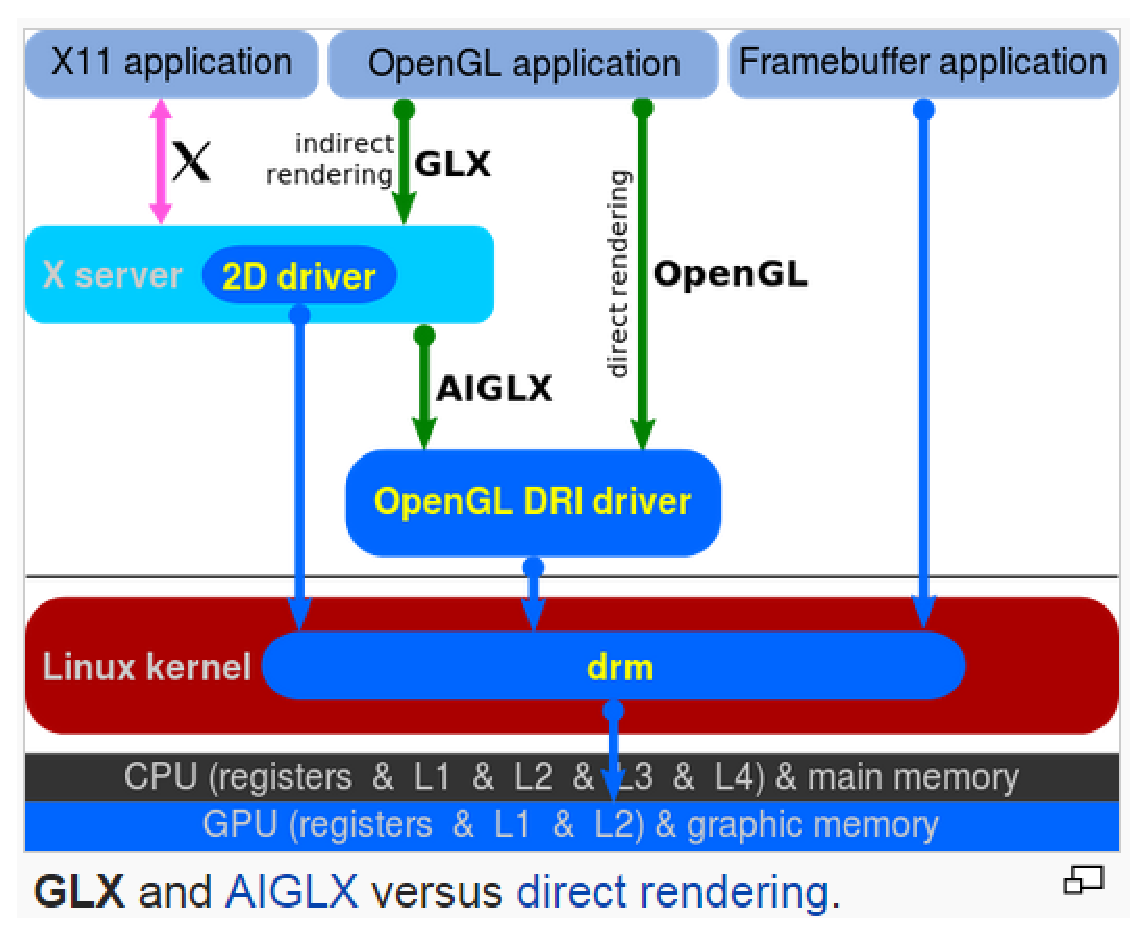
\includegraphics[height=5cm,
    angle=0]{./images/OpenGL_Xserver.eps}}
\caption{{\bf drm} of the kernel control access to the GPU.}
\label{fig:OpenGL_Xserver}
\end{figure}

\subsection{GLX protocol (OpenGL + X11)}
\label{sec:GLX}

{\bf GLX} protocol enables using OpenGL from a window provided by X Windows
System (Sect.\ref{sec:X11}). It provides APIs that connect the OpenGL library
to the X Window System by managing window handles and rendering contexts.
The library is a set of functions and routines that initialize the pixel format,
control rendering, and perform other OpenGL specific tasks.
As of 2011 GLX has reached version 1.4.

The GLX extension was first implemented in XFree86 (Sect.\ref{sec:XFree86}).
\begin{verbatim}
/usr/X11R6/lib/modules/extensions/libglx.a
\end{verbatim}
The part of XServer that renders OpenGL commands for GLX protocol is {\bf
GLcore} - implemented as a software-only version of Mesa, and is used when the
DDX driver does not support DRI. 
\begin{verbatim}
/usr/X11R6/lib/modules/extensions/libGLcore.a
\end{verbatim}
{\bf Utah GLX} is the free early implementation of GLX protocol on Linux-based
O/S, Fig.\ref{fig:XServer_rendering}(2). This was replaced by DRI
implementation.

\subsection{DRI}
\label{sec:DRI}

{\bf DRI} is a framework for allowing direct access to graphics hardware in a
safe and efficient manner.  Without the DRI programs have to perform the
rendering using software.
For example, games or graphics programs can send commands directly to your card
and let it perform fast, hardware-accelerated rendering producing high-quality
visuals. At the same time your CPU is free to do other work. This is known as
direct rendering.

DRI was first made available in XFree86 (Sect.\ref{sec:XFree86}), and is now
part of X11 (Sect.\ref{sec:XServer}).

Initially, the DRI requires a working installation of XFree86 version 4.0.0 or
later, and Linux kernel 2.4.0+. \url{http://dri.sourceforge.net/doc/DRIbeginner.html}
OpenGL-based programs must link with the \verb!libGL! library,
which implements the GLX interface as well as the main OpenGL API entrypoints
(Sect.\ref{sec:GLX}).
\begin{itemize}
  \item When using indirect rendering, libGL creates GLX protocol messages and
  sends them to the X server via a socket. 
  \item When using direct rendering, libGL loads the appropriate 3D DRI driver
  then dispatches OpenGL library calls directly to that driver.
\end{itemize}

The DRI is not a single, isolated piece of software. Instead, the DRI is
composed of a number of distinct modules. 

In 2008 the binding in GLcore to the Mesa software render was rewritten as a DRI
interface module, called \verb!swrast_dri.so!, improving the coupling of Mesa
and the X server. In the same year, a new DRI2 was introduced to replace DRI,
and with it a new model based in the Kernel mode-setting, which uses 
global GEM handles to pass objects (huge securities issues).

DRI3 was proposed in 2012. DRI3 revolves around using POSIX file descriptors for
passing kernel objects between the display server and the application, instead
of passing global GEM handles
\url{http://en.wikipedia.org/wiki/Direct_Rendering_Infrastructure}

To translate these functions in GLX library to Windows: 
\url{https://msdn.microsoft.com/en-us/library/windows/desktop/dd374297(v=vs.85).aspx}

\subsection{AIGLX}
\label{sec:AIGLX}

Accelerated Indirect GLX (AIGLX) brings hardware acceleration to the GLX
(indirect context) applications by loading the Mesa DRI driver inside the X
server, Fig.\ref{fig:XServer_rendering}(4).

\section{OpenGL and Wayland}

Since Linux kernel 3.12, render nodes were introduced,
Fig.\ref{fig:OpenGL_Wayland}.

Wayland (Sect.\ref{sec:Wayland}) implements direct rendering over EGL

\begin{figure}[hbt]
  \centerline{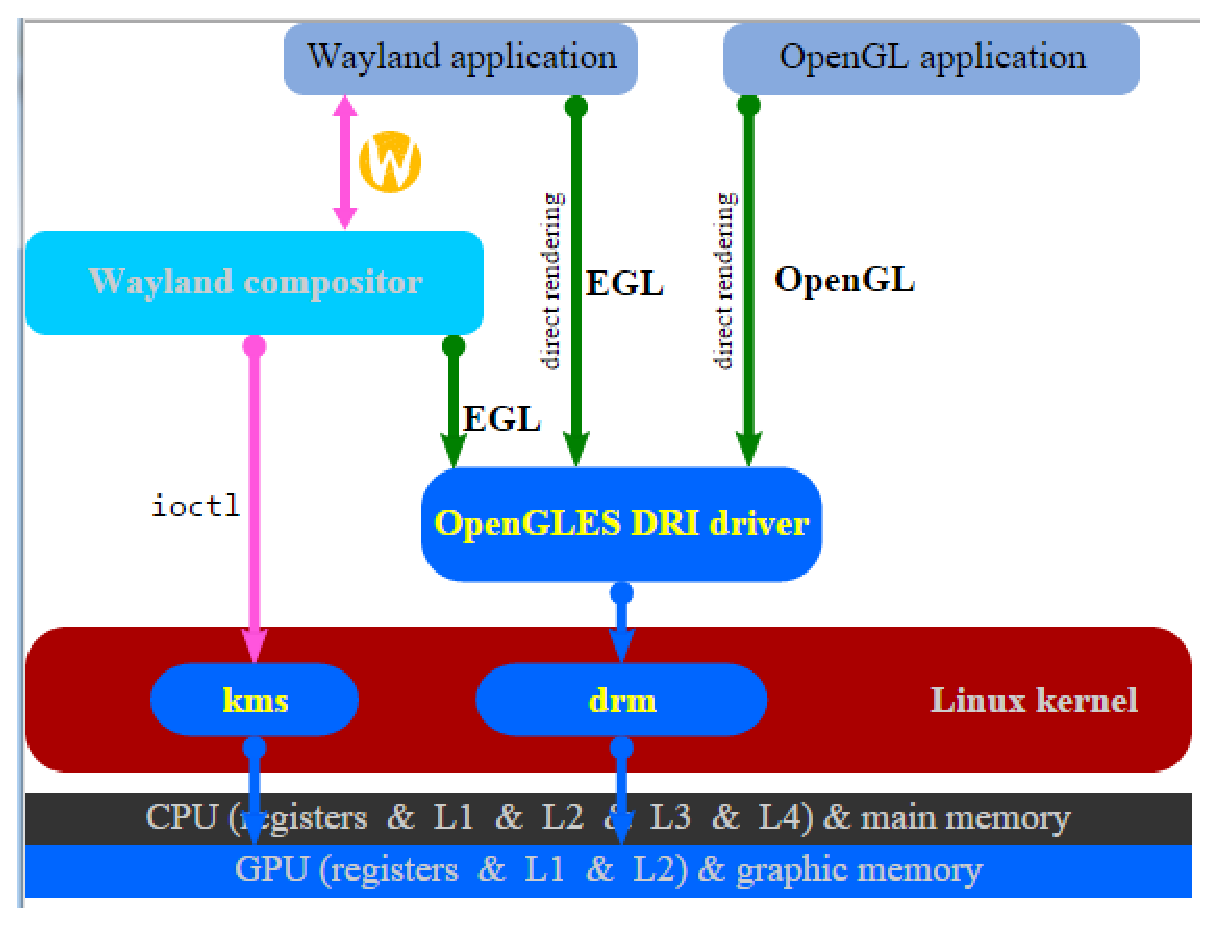
\includegraphics[height=5cm,
    angle=0]{./images/OpenGL_Wayland.eps}}
\caption{OpenGL and Wayland}
\label{fig:OpenGL_Wayland}
\end{figure}



\section{Libraries that use OpenGL}

All OpenGL API-based software/libraries are given in here:
\begin{itemize}
\item \url{http://www.opengl.org/products/platform/C5/P250/}. 
\item  \url{http://www.codemonsters.de/home/content.php?show=freelibraries}

\end{itemize}

All OpenGL functions has \verb!gl!  suffix. Libraries that is built on
top of OpenGL are
\begin{enumerate}
\item \verb!GLU! - Sect.\ref{sec:glu}
 
\item \verb!GLUT! (all function start with \verb!glut! prefix), yet it
  is no longer maintained. Alternative choices are FREEGLUT, SDL,
  OpenML...\footnote{\url{http://www.opengl.org/resources/libraries/windowtoolkits/}}
   
\item \verb!FREEGLUT! : a reimplementation of GLUT

\item \verb!OpenGLUT! : a folk of FREEGLUT

\item \verb!SDL!

\item GUI development: use \verb!GLUI! or \verb!FLTK!

\item Help managing extensions easier: \verb!GLEW! or \verb!GLEE!

\item High-level object-oriented scene graph: \verb!OpenSceneGraph!,
  \verb!OpenSG! ...(commercial product, help creating real-time
  visual simulation application). 
 
\item GLGraphics\footnote{\url{http://glgraphics.sourceforge.net/}}:
  provide a set of classes to simplify the handling of OpenGL texture,
  GLSL shaders and off-screen rendering
\end{enumerate}

GLX (OpenGL GL extensions to the X windows system) integrate
OpenGL with the X Window System. There are different implementation of OpenGL
specification, e.g. GLU (GL Utility), Mesa 3D, GLUT (Chap.{chap:glut}).


\subsection{GLU (for drawing)}
\label{sec:glu}

GLU ({\bf OpenGL Utility Library}) provides a set of higher level drawing
functions implemented on top of OpenGL, i.e.
primitive rendering and mapping between screen- and world-coordinates, etc.

The functions have prefix \verb!glu!. Among these features are
\begin{enumerate}
\item mapping between screen-
  and world-coordinates, 
\item generation of texture mipmaps (MIP maps - a precalculated,
  optimized collections of images that accompany a main texture -
  aimed to improve rendering speed and reduce aliasing artifacts),
\item drawing of quadric surfaces, NURBS (Non-uniform rational
  B-spline), tessellation of polygonal primitives, interpretation of
  OpenGL error codes, 

\item an extended range of transformation routines for setting up
  viewing volumes and simple positioning of the camera, generally in
  more human-friendly terms than the routines presented by OpenGL. 
\end{enumerate}
It also provides additional primitives for use in OpenGL applications,
including spheres, cylinders and disks.

\begin{framed}
  SGI Sample Implementation (SI) include GLU 1.3; while Mesa 3D only
  implements GLU 1.2. So, if you use GLU, it's recommended to install
  SGI SI GLU which is included in the Mesa 3D
  distribution\footnote{\url{http://www.mesa3d.org/glu.html}}.
\end{framed}

\subsection{GLUT (for utilities)}
\label{sec:glut-2}

GLUT ({\bf OpenGL Utility Toolkit}) is a library of utilities for OpenGL.
It contains a set of utilities which focus on window definition, window control
and monitoring of keyboard and mouse input.

Utilities include
\begin{enumerate}
\item functions for window definition, window control, and monitoring
  of keyboard and mouse input.
\item Routines for drawing a number of geometric primitives (both in
  solid and wireframe mode) are also provided, including cubes,
  spheres, and the Utah teapot. GLUT even has some limited support for
  creating pop-up menus.
\end{enumerate}

Any functions of GLUT has the prefix \verb!glut!. GLUT is no-longer
under development, for more information, read Chap.~\ref{chap:glut}. An
alternative choice is freeGLUT (Sect.~\ref{sec:freeglut}).

\subsection{GLEW (loading OpenGL extensions)}
\label{sec:glew}

{\bf OpenGL Extension Wrangler Library} (GLEW) is an opensource multiplatform
library that helps in querying and loading OpenGL Extensions
(Sect.\ref{sec:extensions}).

OpenGL core and extension functionality is exposed in a single header file.
To use GLEW, 
\begin{enumerate}
\item In C/C++: include the file ``GL/glew.h''
\item In Fortran: link to ..., and create an explicit interface to the
  function you want to use
\end{enumerate}

GLEW provides an easy way to get access to the OpenGL extension.  GLEW
can be installed from here:
\url{http://sourceforge.net/projects/glew/}. However, most Linux
distro should have it installed.  

To check for OpenGL extensions being supported, you can use the utility
\verb!glewinfo! (package: glew-utils).

In your code, you can call \verb!glewInit()! and check the error code
\begin{verbatim}
    int err = glewInit();
    // Warning: This does not check if all extensions used
    // in a given implementation are actually supported.
    if (GLEW_OK != err) {
        printf((char*)glewGetErrorString(err));
        exit(ERROR_GLEW);
    }
\end{verbatim}

\begin{enumerate}
\item \verb!glew.h!: OpenGL Extension Wrangler Library that helps
  querying and loading OpenGL extensions. It helps determining which
  extension is supported on your platform

\item \verb!glext.h!: OpenGL Easy Extension Library automatically
  links OpenGL extension and core functions at initialization time
\end{enumerate}

To use in Fortran, you need to link to the library provided in CUDA
SDK
\begin{verbatim}
! 64-bit
-L/usr/local/NVIDIA_GPU_COMPUTING_3.1/C/common/lib/linux/ -lGLEW_x86_64

! 32-bit
-L/usr/local/NVIDIA_GPU_COMPUTING_3.1/C/common/lib/linux/ -lGLEW
\end{verbatim}
NOTE: In CUDA 5.0, the library is renamed, using the same name libGLEW.a for
both 32-bit and 64-bit; yet the file locations are different.
\begin{verbatim}
/usr/local/cuda5.0/samples/common/lib/linux/i686/libGLEW.a
/usr/local/cuda5.0/samples/common/lib/linux/x86_64/libGLEW.a
\end{verbatim}

After linking to the library, then you just define an explicit interface to the
function that you want to use, e.g.
\begin{verbatim}
  INTERFACE
    FUNCTION glewInit() BIND(c, name="glewInit") RESULT(res)
      USE iso_c_binding
      INTEGER(C_INT) :: res
    END FUNCTION glewInit
  END INTERFACE
\end{verbatim}

\url{http://glew.sourceforge.net/install.html}

\section{OpenGL-ES}
\label{sec:OpenGL-ES}

OpenGL-ES (OpenGL for Embedded Systems) is a subset of OpenGL designed for use
on embedded systems like smartphones, tablets, game consoles, etc.

\subsection{WebGL}
\label{sec:WebGL}

Take in mind that they might have the same functions, though WebGL isn't OpenGL
or OpenGL-ES. WebGL is only based on OpenGL-ES.
{\bf WebGL} - based on OpenGL ES 2.0 
provides APIs in JavaScript for 3D rendering on the webbrowser.




\section{Rendering and Coordinate systems}
\label{sec:coordinate-systems}

\begin{figure}[hbt]
  \centerline{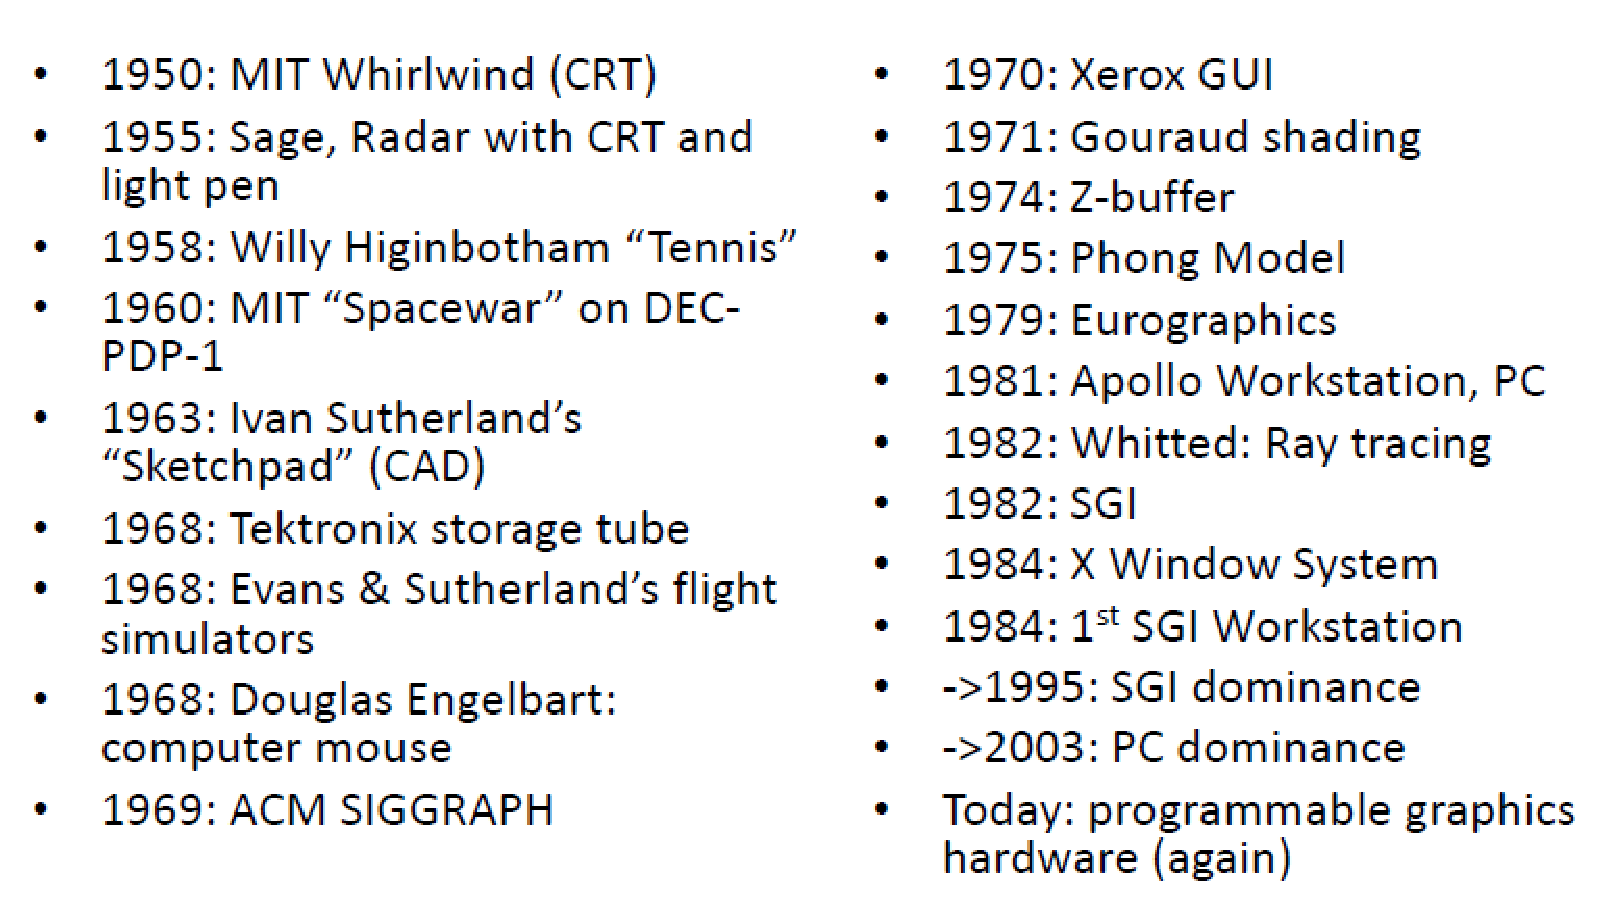
\includegraphics[height=5cm,
    angle=0]{./images/history.eps}}
\caption{History of computer graphics }
\label{fig:history}
\end{figure}

The history of computer graphics is given Fig.\ref{fig:history}.
An object in 3D space is represented via thousands of geometric
primitives (lines, triangles, points). In order to generate a view,
the programmer need to define a ``virtual camera'' and a viewing
angle.  Rasterization takes every vertex, primitives and maps them to
the pixels on the screen.

Before we can describe an object in 3D, we need a coordinate system,
i.e. a frame of reference to measure and locate the object. We have a
number of coordinate system
\begin{enumerate}
\item real world coordinate system (or drawing coordinate): this is
  the system that we define to capture the scene.  The origin is aka
  the location of the ``virtual camera'' and a viewing angle.

\item window coordinate system: this is the system that we define the
  location of objects on the window, the unit is measured in pixels.

\item screen coordinate system: this is the system that we define that
  location of windows on the screen, the unit is measured in pixels,
  e.g. 640x480 in pixels.
\end{enumerate}
These coordinate systems can be based on 
\begin{itemize}
\item 2D Cartesian coordinate, i.e. origin is (x=0,y=0) and the two
  axises are orthogonal. So, how we choose the origin in such system,
  using 2D Cartesian coordinate, will affect the value of the
  coordinate of the objects, Fig.~\ref{fig:clipping}. 
\begin{figure}[hbt]
  \centerline{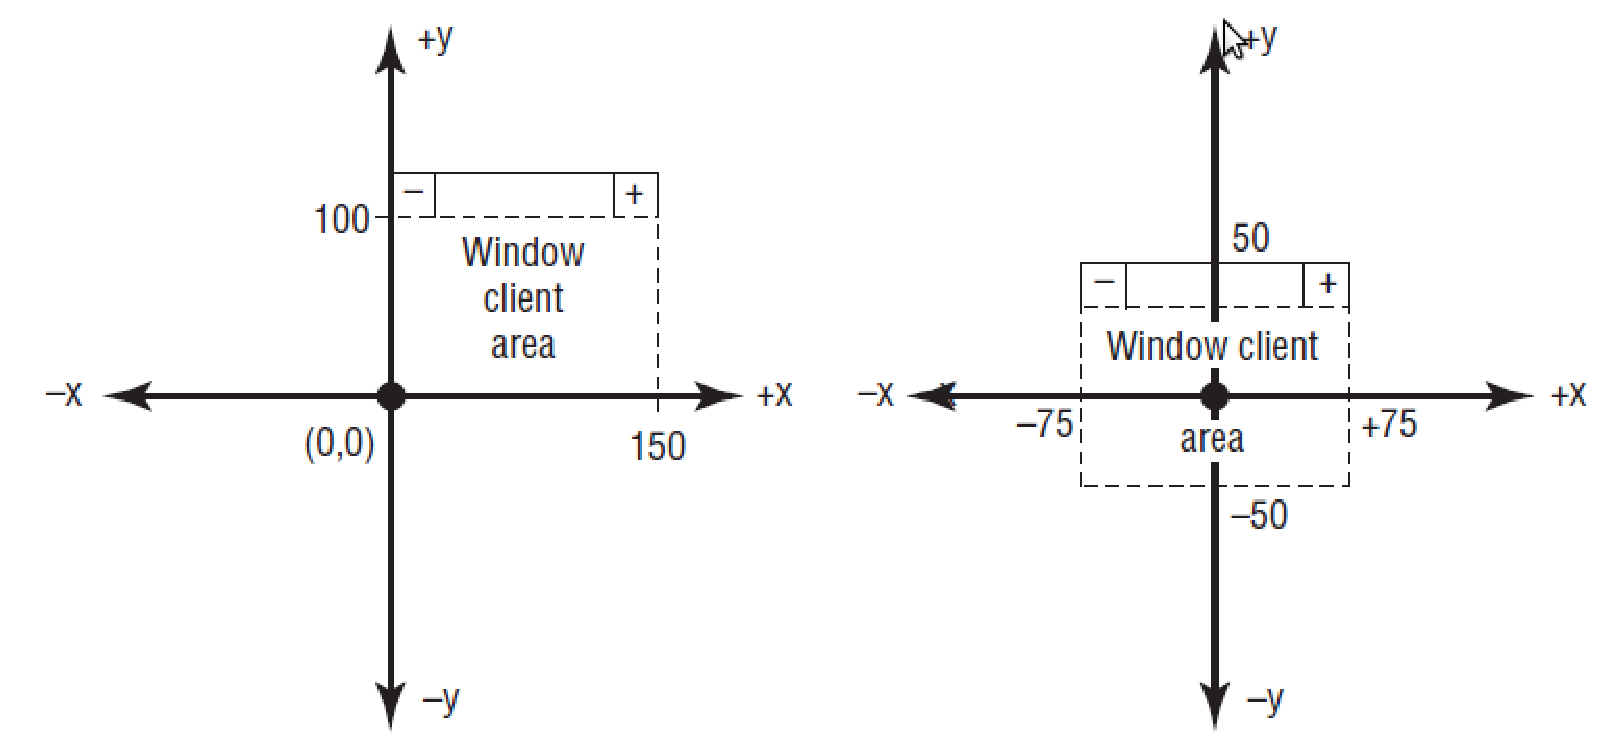
\includegraphics[height=5cm,
    angle=0]{./images/clipping.eps}}
\caption{Two clipping regions}
\label{fig:clipping}
\end{figure}

Using OpenGL we can also turn the coordinate system upside down or
flip it right to left.
\textcolor{red}{In fact, the default mapping for Windows windows is
  for positive $y$ to move down from the top to bottom of the
  window} which is not convenient for drawing graphics. 

You cannot capture the whole real-world, but just a scene of it. This
is known as {\bf clipping}. 

{\bf Viewport}: Rarely, the clipping area of the scene fit the screen
size. So, you need to map from logical Cartesian coordinates to the
area on the physical screen pixel coordinates. This setting is known
as {\bf Viewport}. The viewport is the region within the window on the
physical screen. Normally, the viewport is the entire window, but this
isn't necessary true, Fig.~\ref{fig:viewport}.

\begin{figure}[hbt]
  \centerline{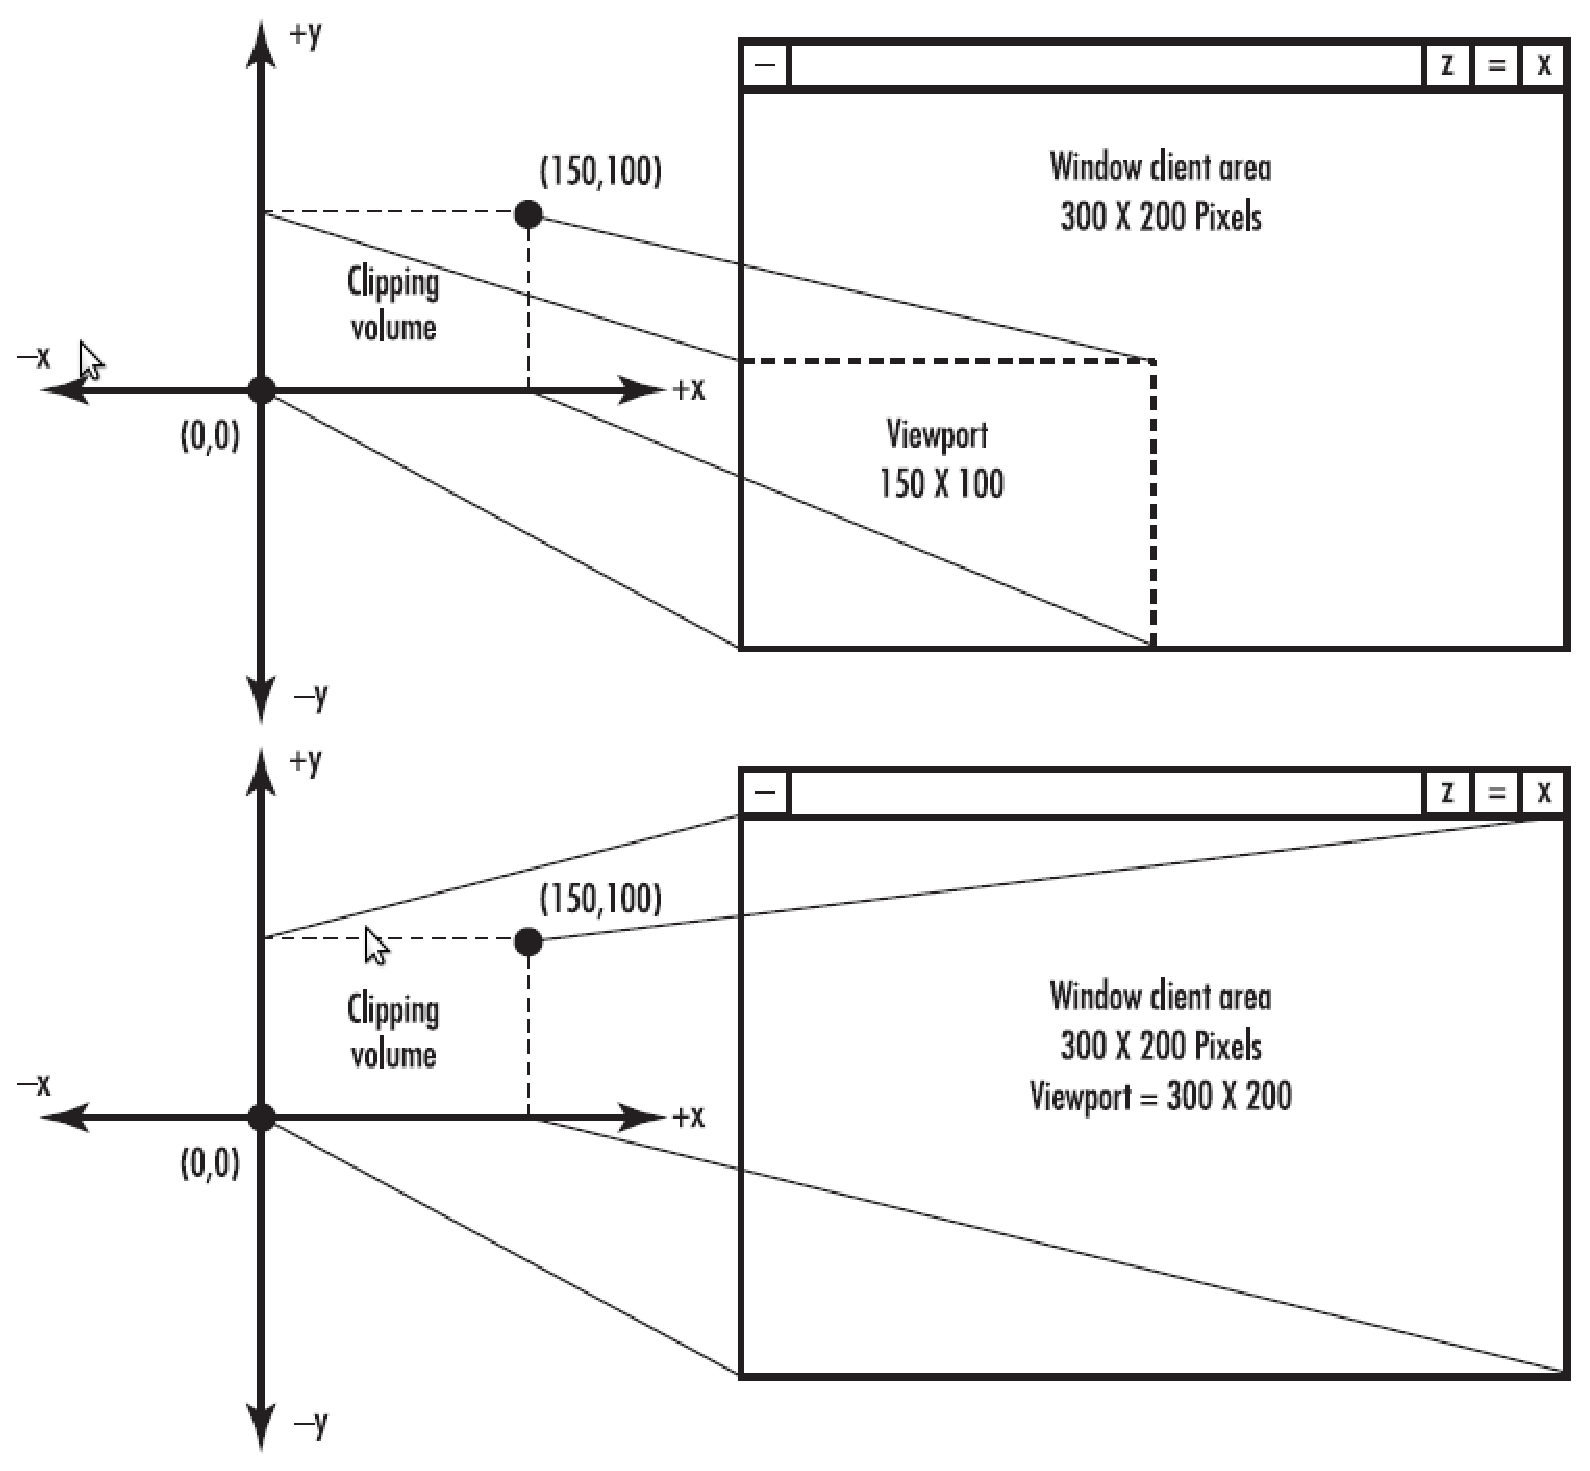
\includegraphics[height=5cm,
    angle=0]{./images/viewport.eps}}
\caption{Two different viewports}
\label{fig:viewport}
\end{figure}

\item 3D Cartesian coordinate, i.e. origin is (x=0, y=0, z=0) and we
  have three axises, orthogonal in pair. Now, instead of a clipping
  area, we have the concept of {\bf clipping volume} (or viewing
  volume, anything outside of this is not drawn).

  So, not only we need to define {\bf viewport}, but also we need to
  define a {\bf projection} which tells how to map 3D coordinates in
  the viewing volume onto a position on the 2D surface. There are two
  ways of projections
  \begin{enumerate}
  \item {\bf orthogonal projection} (or parallel projection),
    Fig.~\ref{fig:orthogonal_projection}: the viewing volume is a
    square or rectangle viewing volume. This type of projection sis
    most often used in architectural design, computer-aided design
    (CAD), or 2D graphs.
\begin{figure}[hbt]
  \centerline{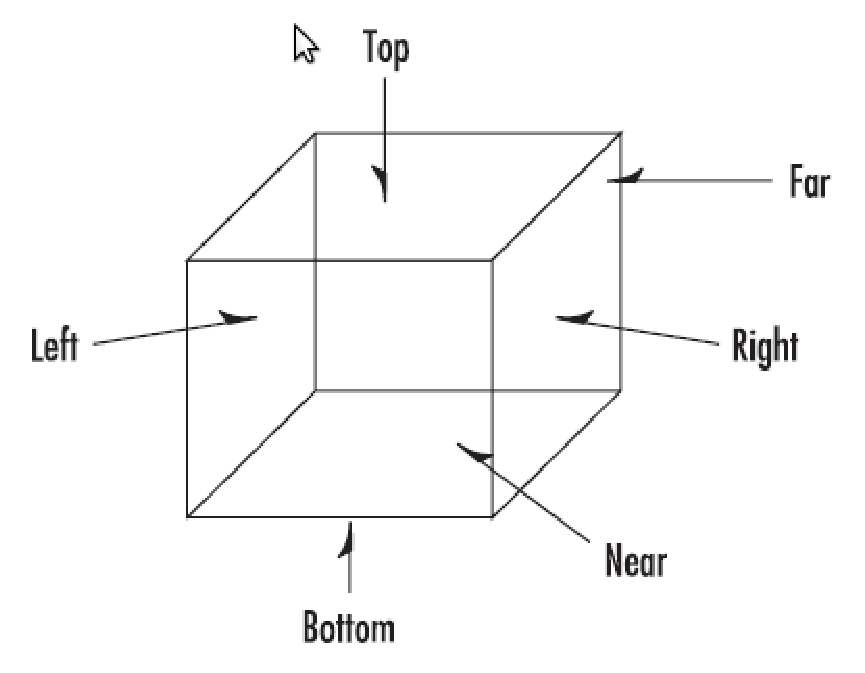
\includegraphics[height=5cm,
    angle=0]{./images/orthogonal_projection.eps}}
  \caption{We need to specify the far, near, left, right, top, and
    bottom clipping planes}
\label{fig:orthogonal_projection}
\end{figure}

\item {\bf perspective projection}: this give you a more realistic
  view, as the size of the planes are different. The clipping volume
  looks like a pyramid with the top shave-off (the shape known as
  {\bf frustum}). Objects near the front of the viewing volume appear
  close to their original size, and those near the back of the viewing
  volume shrink as they are projected on the 2D display,
  Fig.~\ref{fig:perspective_projection}.

\begin{figure}[hbt]
  \centerline{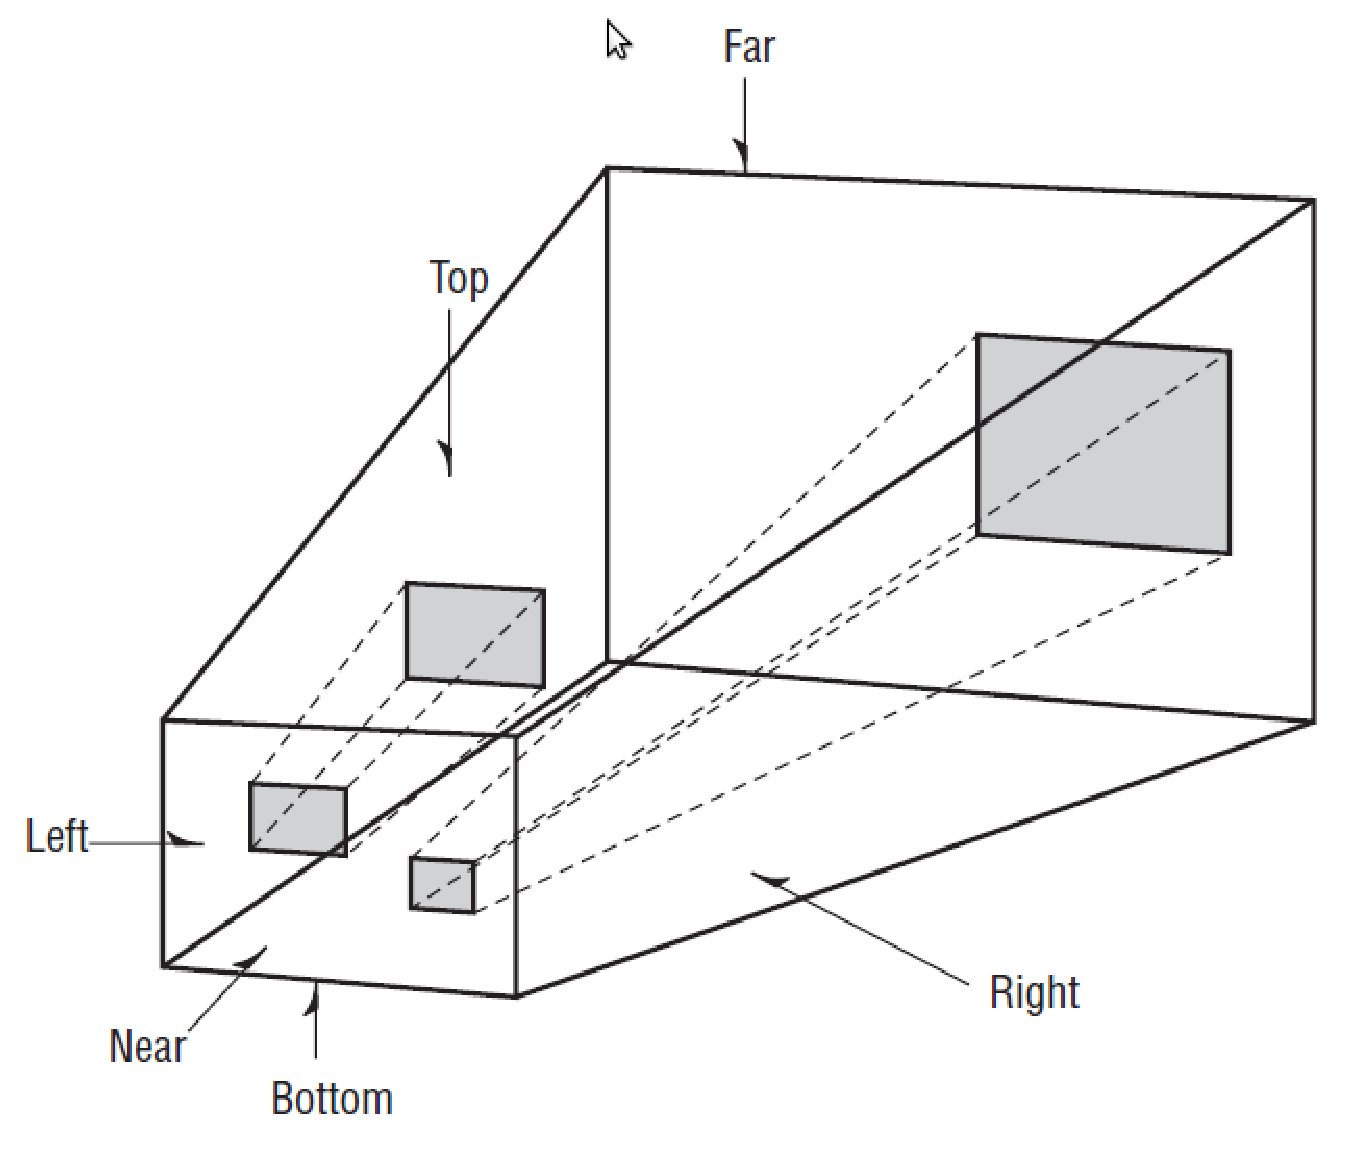
\includegraphics[height=5cm,
    angle=0]{./images/perspective_projection.eps}}
 \caption{Perspective projection}
\label{fig:perspective_projection}
\end{figure}

  \end{enumerate}


\end{itemize}

For more detail, read Sect.~\ref{sec:rendering}. 

% 
% OpenGL is widely used in scientific visualization, CAD, virtual
% reality, video games... Its rival is Direct3D from Microsoft which is
% being used mostly in video games.



\section{GLSL}
\label{sec:GLSL}

GL Shading Language (GLSL).

\section{Shaders}
\label{sec:shaders}

In sect.~\ref{sec:clientserver}, we have learnt that shaders are the
program that run on GPU (not CPU) and do the drawing. The two main types are
vertex shader and pixel shader. The stream of a 3D model flows from application,
to vertex shader, to pixel shader, and finally to the frame buffer
\footnote{\url{http://www.neatware.com/lbstudio/web/hlsl.html}}.
A simple vertex shader program, which receive a data structure (a2v)
transferred from an application to it, the output (v2p) will be given to the
pixel shader:
\begin{verbatim}
  void main(in a2v IN, out v2p OUT, uniform float4x4 ModelViewMatrix) 
  {
    OUT.Position = mul(IN.Position, ModelViewMatrix); 
  }
   
  struct a2v { 
    float4 Position : POSITION; 
  };


  struct v2p {
    float4 Position : POSITION;
  };
    
\end{verbatim}
NOTE: \verb!uniform! modifier indicates that the value of the matrix is a
constant assigned by external program. While IN.Position is the left parameter
of mul, it is considered as a row vector. Otherwise it is considered as a column
vector.  

\begin{framed}
You can think HLSL as a C language for GPU programming except there are no
pointer, union, bitwise operations, and function variables. There are no goto,
switch, recursive function in HLSL as well. However HLSL adds vector data type,
build-in constructor, swizzling and masking operators. HLSL standard library
includes mathematical functions and texture processing functions. The function
overloading has been used to unify the operations of different vectors.  
\end{framed}

The pixel shader does other jobs: adding shading information to the pixel
\begin{verbatim}
  struct v2p {
    float4 Position  : POSITION;
    float2 Texcoord0 : TEXCOORD0;
    float2 Texcoord1 : TEXCOORD1;
    float4 Color     : COLOR0;
  };

  void main( in v2p IN, out p2f OUT ) 
  {  
\end{verbatim}
The output p2f will be given to the frame buffer.



There are some predefined types of shaders. So, we need to load the shader we
want.


\subsection{Identity shader}
\label{sec:identity-shader}

The identity shader simply draws geometry using the default Cartesian
coordinate system (-1.0 to 1.0 on all axes).

A single color is applied to all fragments, and the geometry is solid
and unshaded. The only attribute used is
\verb!GLT_ATTRIBUTE_VERTEX!. The vColor parameter contains the desired
color (RGBA).
\begin{verbatim}
GLShaderManager::UseStockShader(GLT_SHADER_IDENTITY, GLfloat vColor[4]);
\end{verbatim}

\subsection{Flat shader}
\label{sec:flat-shader}

This is more complicated than Identity shader, as it provides a 4x4
matrix \verb!mvp! that can be used to do geometry transformation. This
matrix is often called the modelview projection matrix.

Like identify shader, it use only one attribute
\verb!GLT_ATTRIBUTE_VERTEX!.
\begin{verbatim}
GLShaderManager::UseStockShader(GLT_SHADER_FLAT, 
                       GLfloat mvp[16], GLfloat
                       vColor[4]);
\end{verbatim}


\subsection{Shaded shader (smooth shading)}
\label{sec:shaded-shader}

If this shader is used, colors are interpolated smoothly between the
vertices. You need to enable this shader if you want smooth shading
effect.  Both the \verb!GLT_ATTRIBUTE_VERTEX! and the
\verb!GLT_ATTRIBUTE_COLOR! are used by the shader.

\begin{verbatim}
GLShaderManager::UseStockShader(GLT_SHADER_SHADED, GLfloat mvp[16]);
\end{verbatim}

\subsection{Default Light shader}
\label{sec:default-light-shader}

If you want to have the effect of shade and lit, this shader create
the illusion of a single diffuse light source located at the eye
position (if you want to put the light source at a different position,
use Point Light shader). 

\begin{verbatim}
GLShaderManager::UseStockShader(GLT_SHADER_DEFAULT_LIGHT, 
                 GLfloat mvMatrix[16],
                 GLfloat pMatrix[16], GLfloat vColor[4]);
\end{verbatim}

Most lighting shaders require the normal matrix as a uniform. This
shader derives the normal matrix from the modelview matrix - convenient,
but not terribly efficient. So, not a recommend for
performance-sensitive applications.


Required attributes are \verb!GLT_ATTRIBUTE_VERTEX! and
\verb!GLT_ATTRIBUTE_NORMAL!.

\subsection{Point Light shader}
\label{sec:point-light-shader}

\begin{verbatim}
GLShaderManager::UseStockShader(GLT_SHADER_POINT_LIGHT_DIFF, 
                     GLfloat mvMatrix[16],
                     GLfloat pMatrix[16], 
                     GLfloat vLightPos[3], //light source
                     GLfloat vColor[4]);
\end{verbatim}

\subsection{Texture Replace shader}
\label{sec:text-repl-shad}

\begin{verbatim}
GLShaderManager::UseStockShader(GLT_SHADER_TEXTURE_REPLACE,
GLfloat mvpMatrix[16], GLint nTextureUnit);
\end{verbatim}

\subsection{Texture Modulate shader}
\label{sec:text-modul-shad}

\begin{verbatim}
GLShaderManager::UseStockShader(GLT_SHADER_TEXTURE_MODULATE, 
             GLfloat mvpMatrix[16],
             GLfloat vColor, GLint nTextureUnit);
\end{verbatim}

\subsection{Textured Point Light shader}
\label{sec:textured-point-light}

\begin{verbatim}
GLShaderManager::UseStockShader(GLT_SHADER_TEXTURE_POINT_LIGHT_DIFF,
    GLfloat mvMatrix, GLfloat pMatrix[16], GLfloat vLightPos[3],
    GLfloat vBaseColor[4], GLint nTextureUnit);
\end{verbatim}

Above are pre-defined shaders. Users nowadays can write their own
shaders. 

\section{2D Array = Texture = Pixmap}
\label{sec:arrays-=-textures}

Native memory layout in CPU is in 1D. Any higher dimensional array
will eventually mapped to 1D by the compiler. 
However, in GPU, native data layout is 2D. 1D and 3D arrays are also
supported in GPU, however they may impose a performance penalty.

\begin{framed}
  A texture is an image (2D) that can be applied to a triangle in your
  scene - the process known as {\bf texture mapping}. So the solid
  area is filled with {\bf texels} - the texture-based equivalent of
  pixel.

  Original electronic computer display data in monochrome (one color)
  with each pixel can receive on or off value (0 or 1). So an image is
  represented as a {\bf bitmap} - a series of 1s and 0s (in 1D). 

  In grayscale images, each pixel can receive one of 256
  values. Windows has the .BMP file extension that hold this picture
  file format.The image with each pixel represented by more than one
  bit is called {\bf pixmap} (pixel rectangle).
\end{framed}

\subsection{Front/Back and other buffers}
\label{sec:frontb-other-buff}

OpenGL stores and manipulates pixel data in a framebuffer. The
framebuffer is not a real buffers as it doesn't contain data. It
indeed serves as a container that hold other buffers, e.g. color
buffer, depth buffer, accumulation buffer and stencil buffers. It is
these buffers that hold true data. 

The color buffer contains a set of logical buffers (front-left,
front-right, back-left, back-right and some number of auxiliary
buffers). An implementation OpenGL many not supply all of these
buffers. However, most implementations support {\bf double buffering
  of images}. This is a technique in which an application draw pixels
to an off-screen buffer, and then when that image is ready for
display, the application copies the content of the off-screen buffer
to an on-screen buffer. Double buffering enables smooth image changes,
which is especially important for animated images. GLUT/FreeGLUT
help make it easier for user by providing
\begin{enumerate}
\item \verb!GLUT_DOUBLE! option
\item \verb!glutSwapBuffers()! function (call when the off-screen
  buffer is ready for display)
\end{enumerate}

In Windows, we set \verb!PFD_DOUBLEBUFFER! flag in the
PIXELFORMATDESCRIPTOR data structure. 

When color are written to a framebuffer, they are written to the color
buffer specified by \verb!glDrawBuffer()!. Even though you can write
to a single color buffer at a time, you can select more than one color
buffer (with written data) for drawing. This help creating {\bf
  blending effect}. .

\subsection{Pixel packing}
\label{sec:pixel-packing}

Image data is rarely packed tightly into memory. The reason is that
each row of an image should start at some particular byte-aligned
address for optimal performance. OpenGL use 4-byte alignment. So, it's
best to use RGBA for a pixel. 

.BMP use 4byte-aligned format; yet .TGA use 1byte-aligned format. You
can change how tightly packed pixel data using
\begin{verbatim}
// tell how OpenGL unpack data from data buffers
glPixelStorei(GL_UNPACK_ALIGNMENT, 1);

// tell how OpenGL pack data being read from pixel buffers
// and place them into a user-specified memory buffer
glPixelStorei(GL_PACK_ALIGNMENT, 1);


// syntax:
void glPixelStorei(GLenum pname, GLint param);
void glPixelStoref(GLenum pname, GLfloat param);
\end{verbatim}

\subsection{Pixmap}
\label{sec:pixmap}

We cannot draw a pixmap directly into the color buffer but you can
read the content of the color buffer directly as a pixmap. This data
is copied back to the client side memory during which your application
is blocked until the transfer has completed (for GPU-to-GPU memory
copy, read Sect.~\ref{sec:buffer-objects} and
Sect.~\ref{sec:cuda-app.-with}). In addition, if you specify a pixel
layout different from the native arrangement of your graphics
hardware, there will be an additional performance penalty as the data
is reformatted.
\begin{verbatim}
void glReadPixels(GLint x, GLint y, GLSizei width, GLSizei height,
GLenum format, GLenum type, const void *pixels);
\end{verbatim}
with the x and y in window coordinates of the lower-left corner of the
rectangle to read followed by width and height of the rectangle in
pixels. If the color buffer stores data differently than what you have
requested, OpenGL takes care of the necessary conversions.  This
capability can be very useful. The pointer to the image data, *pixels,
must be valid and must contain enough storage to contain the image
data after conversion, or you will likely get a nasty memory exception
at runtime. Also be aware that if you specify window coordinates that
are out of bounds, you will get data only for the pixels within the
actual OpenGL frame buffer. The fourth argument specify the color
layout, which can be any thing in Table.~\ref{tab:OpenGL_color}. The
fifth argument tell the type for each color component,
Table~\ref{tab:pixel_data_type}. 


For our glReadPixels function, by default, the read operation is
performed on the back buffer for double-buffered rendering contexts,
and the front buffer for single-buffered rendering contexts. You can
change the source of these pixel operations by using this function:
\begin{verbatim}
void glReadBuffer(GLenum mode);
\end{verbatim}
The mode parameter can be any one of 
\begin{verbatim}
GL_FRONT, GL_BACK, GL_LEFT, GL_RIGHT,
GL_FRONT_LEFT, GL_FRONT_RIGHT, GL_BACK_LEFT, 
GL_BACK_RIGHT, or even GL_NONE.
\end{verbatim}


\subsection{Loading texture (1D, 2D, 3D)}
\label{sec:loading-texture}

The first step before you can write a texture to a solid area is to
load the texture (image data) (e.g. from a disk file) into the memory.
\begin{verbatim}
void glTexImage1D(GLenum target, GLint level, GLint internalformat,
       GLsizei width, GLint border,
       GLenum format, GLenum type, void *data);

void glTexImage2D(GLenum target, GLint level, GLint internalformat,
       GLsizei width, GLsizei height, GLint border,
       GLenum format, GLenum type, void *data);

void glTexImage3D(GLenum target, GLint level, GLint internalformat,
       GLsizei width, GLsizei height, GLsizei depth, GLint border,
       GLenum format, GLenum type, void *data);
\end{verbatim}
OpenGL supports one-, two-, and threedimensional texture maps and uses
the corresponding function to load that texture and make it
current. This data copy can be quite expensive.

The target argument for these functions should be
\verb!GL_TEXTURE_1D!, \verb!GL_TEXTURE_2D!, or \verb!GL_TEXTURE_3D!,
respectively. You may also specify proxy textures by specifying
\begin{verbatim}
GL_PROXY_TEXTURE_1D, GL_PROXY_TEXTURE_2D, or GL_PROXY_TEXTURE_3D 
\end{verbatim}
using the function \verb!glGetTexParameter()! to retrieve the results
of the proxy query (read Sect.~\ref{sec:proxy-texture}). 

The \verb!level! tells the mipmap level being loaded (for non-mipmap,
set it to 0) (read Sect.~\ref{sec:mipmap-generation}).

The \verb!internalformat! parameter of the texture data. This
information tells OpenGL how many color components you want stored per
texel and possibly the storage size of the components and/or whether
you want the texture compressed,
Table~\ref{tab:texture_internal_format}.

\begin{framed}
  The width, height, and depth parameters (where appropriate) specify
  the dimensions of the texture being loaded. It is important to note
  that prior to OpenGL 2.0, these dimensions must be integer powers of
  2 (1, 2, 4, 8, 16, 32, 64, and so on). 

  There is no requirement that texture maps be square (all dimensions
  equal), but a texture loaded with non-power of 2 dimensions on older
  OpenGL implementations will cause texturing to be implicitly
  disabled. Even though OpenGL 2.0 (and later) allows non-power of 2
  textures, this is no guarantee that they will necessarily be fast on
  the underlying hardware. Many performance-minded developers still
  avoid non-power of two textures for this reason.
\end{framed}
.

\begin{table}[hbt]
\begin{center}
\caption{Texture internal format}
\begin{tabular}{cc} 
\hline
\verb!GL_ALPHA!& Store the texels as alpha values\\
\verb!GL_LUMINANCE!& Store the texels as luminance values\\
\verb!GL_LUMINANCE_ALPHA! & Store the texels with both luminance and alpha values\\
\verb!GL_RGB!& Store the texels as red, green, and blue components\\
\verb!GL_RGBA! & Store the texels as red, green, blue, and alpha components\\
\hline\hline
\end{tabular}
\end{center}
\label{tab:texture_internal_format}
\end{table}

The border parameter allows you to specify a border width for texture
maps. Texture borders allow you to extend the width, height, or depth
of a texture map by an extra set of texels along the borders. Texture
borders play an important role in the discussion of texture filtering
to come. For the time being, always set this value to 0 (zero).


The last three parameters ``format, type, and data" are identical to the
corresponding arguments when you used glReadPixels in the previous
section. 

\subsection{Proxy texture}
\label{sec:proxy-texture}



\subsection{Cubemap texture}
\label{sec:cubemap-texture}


Arrays in GPU is called {\bf textures} or {\bf texture samplers}.
Texture dimensions are limited on GPUs, the maximum value in each
dimension can be queried with a bit of code like this once a valid
OpenGL context is available (that is, once GLUT is initialized). On
today's graphics card, the maximum range is 2048 or 4096 per
dimension.

\begin{verbatim}
int maxtexsize;

glGetIntegerv(GL_MAX_TEXTURE_SIZE,&maxtexsize);

printf("GL_MAX_TEXTURE_SIZE, %d\n",maxtexsize);   
\end{verbatim}


In CPU, we usually talk about {\bf array indices}. In GPU, however, we
use {\bf texture coordinates} to get access to the value stored in the
textures with the notation is S, T, and R. Texture coordinates need to
address texel centers.

\begin{framed}
  Traditionally, GPUs work on four-tupels of data simultaneously:
  There are four color channels called red, green, blue and alpha
  (RGBA). We will explain later on how we can exploit this to speed up
  our implementation on certain hardware.
\end{framed}


\textcolor{red}{Working with texture is easy once we know texture
  target, texture format and internal format} we want to use:

\begin{enumerate}
\item (named texture) To create a named texture
\begin{verbatim}
GLuint texture;

// allocate a texture name
glGenTextures( 1, &texture );
\end{verbatim}
  use a value higher than 1 if you want to create an array of
  continuous texture names.  The named textures are unsigned integers,
  with the value zero is reserved to represent the default texture for
  each texture target.

\item (texture target) This texture name can be used to bind to any texture target
  using \verb!glBindTexture! function. 
\begin{verbatim}
void glBindTexture(GLenum  target, 
                   GLuint  texture);
\end{verbatim}
  When a texture is bound to a target, the previous binding for that
  target is automatically broken. 
  
  In OpenGL, there are two common forms of texture targets: 1D
  (\verb!GL_TEXTURES_1D!) and 2D (\verb!GL_TEXTURE_2D!) with the
  latter one is more common.  When a named texture bind to
  \verb!GL_TEXTURE_1D!, it becomes a 1D texture; if it bind to
  \verb!GL_TEXTURE_2D!, it becomes a 2D textures...

  \textcolor{red}{The limitation for current OpenGL textures is that
    they requires power-of-two sized dimensions (POTS)},
  e.g. 16, 32, 64... So, resampling is required to convert data to the
  correct dimensions. For non-power-of-two sized textures, read
  Sect.~\ref{sec:nopts-texture}.
\begin{verbatim}
// select our current texture
glBindTexture( GL_TEXTURE_2D, texture );
\end{verbatim}

\item Optional:
  \begin{enumerate}
  \item \verb!glGetBoolean! with \verb!GL_TEXTURE_1D! /
    \verb!GL_TEXTURE_2D! / etc to check whether texture is enabled for
    that dimension. 
  \item \verb!glGetInteger()! to query which texture name is currently
    bound to a particular dimension(beware this used to be an
    extension, so I'm not sure it will be available by default under
    Windows).
  \end{enumerate}

\item Set some texture environment variables
\begin{verbatim}
// select modulate to mix texture with color for shading
glTexEnvf( GL_TEXTURE_ENV, GL_TEXTURE_ENV_MODE, GL_MODULATE );
\end{verbatim}
  \verb!GL_MODULATE! simply takes the color and alpha data from the
  texture and multiplies it with the color data from glColor and/or
  the lighting system.


\item Set some texture parameters which allows us to use wonderful
  effects like bilinear and trilinear texture filtering, and
  mipmapping. 
\begin{verbatim}
// when texture area is small, bilinear filter the closest mipmap
glTexParameterf( GL_TEXTURE_2D, GL_TEXTURE_MIN_FILTER,
                 GL_LINEAR_MIPMAP_NEAREST );
// when texture area is large, bilinear filter the original
glTexParameterf( GL_TEXTURE_2D, GL_TEXTURE_MAG_FILTER, GL_LINEAR );

// the texture wraps over at the edges (repeat)
glTexParameterf( GL_TEXTURE_2D, GL_TEXTURE_WRAP_S, GL_REPEAT );
glTexParameterf( GL_TEXTURE_2D, GL_TEXTURE_WRAP_T, GL_REPEAT );
\end{verbatim}
  We also can setup whether the texture wraps over at the edges or is
  clamped at the ends. We'll stick to repeating because that is the
  most common use. Just read the comments for details on what each
  does.
  \begin{itemize}
  \item For clamped textures, S \& T are in the range of 0 to 1.
  \item For repeated textures, the range is 0 to 1 for every repeat of
    the texture, as is 1 to 2, 2 to 3, and even -1 to 0. Just feed the
    coordinates much like a glColor command, only use the glTexCoord.

  \end{itemize}
  \begin{framed}
    Just remember, any color you fed to glColor is multiplied by the
    texture data, so if your texture is dark or an unusual color,
    check to see what color you are setting to.
  \end{framed}

\item Load the texture data
\begin{verbatim}
/* Suppose the data is RAW */
BYTE * data;
// texture data
width = 256;
height = 256;

data = malloc( width * height * 3 );
// load data into data (in some way)
// or compute the first data
// here, suppose data is from file
    // open texture data
    file = fopen( filename, "rb" );
    if ( file == NULL ) return 0;
    // read texture data
    fread( data, width * height * 3, 1, file );
    fclose( file );
\end{verbatim}
  You could load from PCX, BMP, GIF, JPG, or any other file
  format. You just have to load the image data for OpenGL, and let it
  do the rest. 

\item (Use if mipmap is enable) we create a mipmap. There a function
  to do that, all we need todo is feed it some information on the
  image and the actual image data and it does all the work for us.
\begin{verbatim}
/* Now we can build the texture mipmap */
gluBuild2DMipmaps( GL_TEXTURE_2D, 3, width, height,
                   GL_RGB, GL_UNSIGNED_BYTE, data );
/* free buffer (if we don't need it)
   the mipmap (image data) has been copied to the OpenGL system
*/
free( data );
\end{verbatim}

\item Enable texture mapping
\begin{verbatim}
glEnable( GL_TEXTURE_2D );
\end{verbatim}

\item (internal format) GPUs allow for the simultaneous processing of
  scalars, tupels, tripels or four-tupels of data. In this tutorial,
  we focus on scalars and four-tupels exemplarily. The easier case is
  to allocate a texture that stores a single floating point value per
  texel, i.e. \verb!GL_LUMINANCE!.

\item Now, we specify the 2D texture image
\begin{verbatim}
glTexImage2D(texture_target, 0, internal_format,
             texSize, texSize, 0, texture_format, GL_FLOAT, 0);
\end{verbatim}
The second parameter set to 0 means we don't need to use mipmaps
levels for this texture (i.e. do not create miniature copies). 

The sixth parameter set to 0 means we don't need border (turn off border)

\item Callback\footnote{\url{http://www.nullterminator.net/gltexture.html}}
\begin{verbatim}
glBegin( GL_QUADS );
glTexCoord2d(0.0,0.0); glVertex2d(0.0,0.0);
glTexCoord2d(1.0,0.0); glVertex2d(1.0,0.0);
glTexCoord2d(1.0,1.0); glVertex2d(1.0,1.0);
glTexCoord2d(0.0,1.0); glVertex2d(0.0,1.0);
glEnd();
\end{verbatim}


\item Free the texture
\begin{verbatim}
glDeleteTextures( 1, &texture );
\end{verbatim}
\end{enumerate}

\begin{verbatim}
// create a new texture name
GLuint texID;
glGenTextures (1, &texID);

// bind the texture name to a texture target
// replace texture_texture with appropriate value
glBindTexture(texture_target,texID);

// turn off filtering and set proper wrap mode
// (obligatory for float textures atm)
glTexParameteri(texture_target, GL_TEXTURE_MIN_FILTER, GL_NEAREST);
glTexParameteri(texture_target, GL_TEXTURE_MAG_FILTER, GL_NEAREST);
glTexParameteri(texture_target, GL_TEXTURE_WRAP_S, GL_CLAMP);
glTexParameteri(texture_target, GL_TEXTURE_WRAP_T, GL_CLAMP);

// set texenv to replace instead of the default modulate
glTexEnvi(GL_TEXTURE_ENV, GL_TEXTURE_ENV_MODE, GL_REPLACE);

// and allocate graphics memory
glTexImage2D(texture_target, 0, internal_format,
             texSize, texSize, 0, texture_format, GL_FLOAT, 0);
\end{verbatim}


The strength of using OpenGL 2D texture over \verb!glDrawPixels! is
that linear filtering can be selected.

\url{http://pinyotae.blogspot.com/2010/06/gltexture2d.html}

\subsection{GL\_TEXTURE\_2D}
\label{sec:gl_texture_2d}

Using texture 2D
\begin{enumerate}
\item dimensions are constrained to the power of 2, e.g. 1024-by-512, 
with an optional 1-texel border

\item 
\end{enumerate}




\subsection{GL\_TEXTURE\_3D}
\label{sec:gl_texture_3d}

\begin{verbatim}
glEnable(GL_TEXTURE_3D);
\end{verbatim}

The next, not-so-obvious step is we 


\url{http://gpwiki.org/index.php/OpenGL:Tutorials:3D_Textures}

\subsection{GL\_TEXTURE\_CUBE\_MAP}
\label{sec:gl_texture_cube_map}

This is a cubed-mapped texture target. 

\subsection{NPOTS texture}
\label{sec:nopts-texture}


Non-power-of-two sized (NPOTS) textures are useful for storing video
images that do not have power-of-two sized (POTS).  Re-sampling
artifacts are avoided and less texture memory may be required by
using non-power-of-two sized textures.  

\verb!ARB_texture_non_power_of_two! extension relaxes the size
restrictions for the 1D, 2D, cube map, and 3D texture targets.
\begin{enumerate}
\item Are cube map texture images still required to be square when this
  extension is supported? - YES. As long as width and height are the
  same, they can be NPOT. 
\end{enumerate}

Non-power-of-two sized textures are also useful for shadow maps and
window-space texturing.  However,
\textcolor{red}{non-power-of-two sized textures have limitations that
  do not apply to power-of-two sized textures}.
Another difference is NPOTS textures may not use mipmap filtering;
POTS textures support both mipmapped and non-mipmapped filtering.

\subsection{GL\_TEXTURE\_RECTANGLE\_ARB}
\label{sec:gl_t}

Rectangular texture is an entire new texture target type.  The texture
rectangle target relaxes the power-of-two dimensions requirements of
the texture 2D target, yet it also has limitations such as the absence
of both mipmapping and the \verb!GL_REPEAT! and
\verb!GL_MIRRORED_REPEAT! wrap modes.  

Even though \verb!GL_TEXTURE_RECTANGLE_ARB! relaxes the power-of-two
requirement, it is not classsfied into NPOTS textures. The reason is
that
\begin{enumerate}
\item NPOTS (as well as conventional targets) use normalized texture
  coordinates (ie, [0..1]), while the texture rectangle target uses
  unnormalized (ie, [0..w]x[0..h]) texture coordinates.

\item MIPMAPPING is allowed in NPOTS, yet it's not in texture
  rectangle with default filter is LINEAR. 

\item NPOTS supports borders, which is not available in texture
  rectangle

\item NPOTS doesn't supported palette textures, which is supported by
  textures rectangle

\item NPOTS support all wrap modes; while textures rectangle only
  support CLAMP* wrap modes. 
\end{enumerate}

\subsection{Texture border}
\label{sec:texture-border}

Texture border is particularly useful when you try to render a large
image that doesn't fit into a single texture map. In this case, the
texture need to be broken up into tiles, each with a one-pixel wide
border from the neighboring tiles. For example, a 1024-by-1024 texture
is broken up into four 512-by-512 images which correspond to the
texture coordinate ranges (0-0.5,0-0.5), (0.5,1.0,0-0.5),
(0-0.5,0.5,1.0) and (.5-1.0,.5-1.0).

The key to understanding texture borders is understanding how textures
are sampled when the texture coordinate values are near the edges of
the [0,1] range. {\bf Wrap mode} is the mechanism that you use to tell
how OpenGL process to use (1) a constant texture border color or (2) a
border that is a portion of the edge of the texture image, or (3) ...
There are 5 wrap modes
\begin{enumerate}
\item \verb!GL_REPEAT! (default): 

\item \verb!GL_CLAMP!:

\item \verb!GL_CLAMP_TO_EDGE!: 

\item \verb!GL_CLAMP_TO_BORDER!:

\item \verb!GL_MIRRORED_REPEAT!: 
\end{enumerate}

You call
\begin{verbatim}
glTexParameteri(GL_TEXTURE_2D, GL_TEXTURE_WRAP_S, GL_REPEAT);
\end{verbatim}
The second argument can be \verb!..._S, ..._T, ..._R!. 

\url{http://www.opengl.org/resources/code/samples/sig99/advanced99/notes/node64.html}

\subsection{Mipmap generation}
\label{sec:mipmap-generation}

Mipmapping is a powerful texturing technique that can improve both the
rendering performance and the visual quality of a scene. It does this
by addressing two common problems with standard texture mapping. T

The previous section describes using tiles to generate high resolution
images 

\url{http://www.opengl.org/resources/code/samples/sig99/advanced99/notes/node65.html}


References:
\begin{enumerate}
\item \url{http://www.nullterminator.net/gltexture.html}
\item
  \url{http://www.opengl.org/registry/specs/ARB/texture_rectangle.txt} 
\item
  \url{http://www.opengl.org/registry/specs/ARB/texture_non_power_of_two.txt} 
\end{enumerate}


\section{PPM vs. PGM}
\label{sec:ppm-vs.-pgm}

References:
\begin{itemize}
\item \url{http://www.physics.emory.edu/~weeks/graphics/mkppm.html}
\end{itemize}
\subsection{PPM (Portable Pixel Map)}
\label{sec:ppm-portable-pixel}

PPM is the format being used to make wonderful color (and black/white)
pictures. You use this format if the picture is a rectangle and you
want to specify the exact color for each pixel. 

The top 3 lines are
\begin{verbatim}
P3
# comment line -- whatever you want
100 200
255 
\end{verbatim}
\begin{itemize}
\item P3 = ASCII color file (P6 = binary color file)
\item the second line = can be any thing
\item third line = width + height of the picture (pixels)
\item fourth line = 255 (the maximum intensity of the picture),
  i.e. you use 0-255 to specify the intensity for RGB
\item next = data telling Red/Green/Blue triples for each pixel (in
  row-order
\end{itemize}

\begin{verbatim}
int x,y; int width,height,red,green,blue; 
printf("P6\n"); 
printf("#created by Eric R. Weeks using a C program\n"); 
printf("%d%%d\n",width,height); 
printf("255\n");
            %%/* Do this for the whole picture now
            %%*/ 
for (y = 0;y < height;y++) { 
  for (x = 0;x < width;x++) {
               . . . 
     fputc((char)red,stdout);
     fputc((char)green,stdout);
     fputc((char)blue,stdout); } 
  } 
}
\end{verbatim}

\subsection{PGM (Portable Grey Map)}
\label{sec:pgm-portable-grey}

This is the same as PPM, with using P2 = ASCII black/white file (P5 =
binary black/white file) and the format is called Portable Grey Map
(PGM)


\section{Rendering}
\label{sec:rendering}


\subsection{Ortho vs. Perspective (camera) mode}
\label{sec:ortho-vs.-persp}

Sect.~\ref{sec:coordinate-systems} has provided some basic
information. OpenGL provides function to set the ortho or perspective
mode. GLUT also provides two corresponding functions:
\verb!gluPerspective()! and \verb!gluOrtho2D()!.

\begin{enumerate}
\item In ortho mode your camera behaves like a square or rectangle box
  around the origin. So, the object keeps their dimensions and size
  even if they far away from the camera, so more fillrate is needed.

\item In perspective the camera behaves like a cut-off pyramid with
  the tip being the eye (first 3 floats). This mode give you a
  realistic view of the scene, i.e. the farther an object is from the
  camera, the smaller it looks, so less fillrate is needed to color
  it.

  We can use \verb!gluLookAt()! to place our ``eyes'' at any point in
  space and look at any other point.
\end{enumerate}

\begin{figure}[hbt]
  \centerline{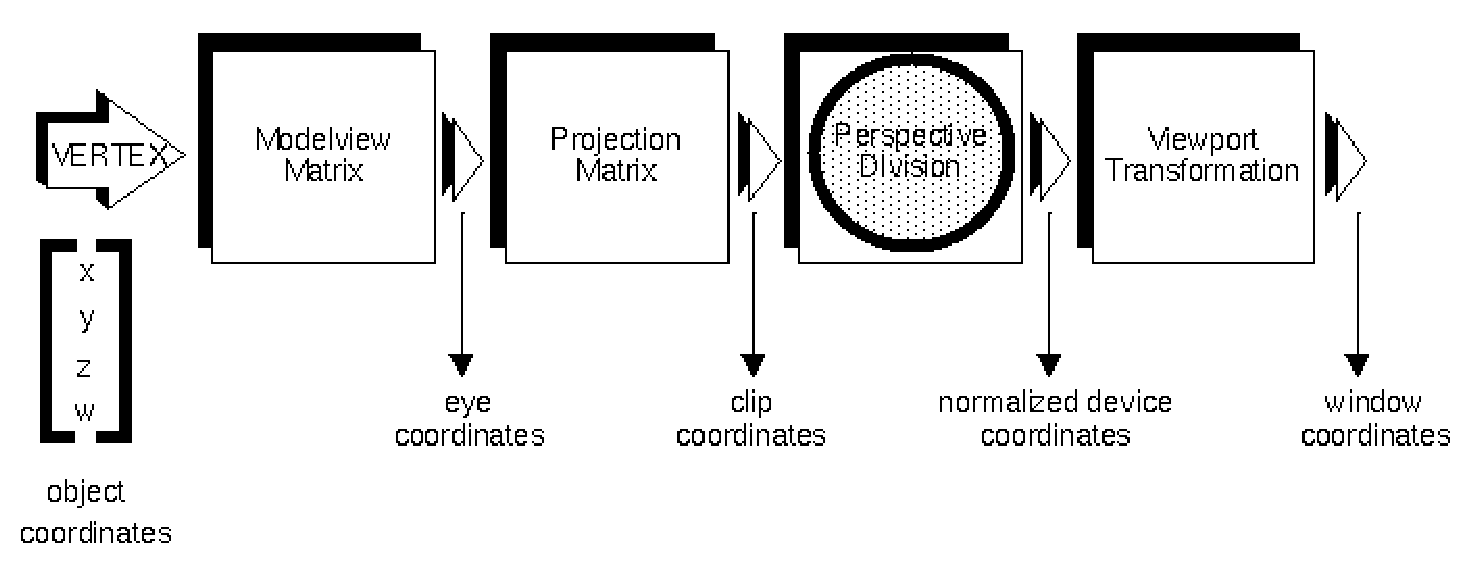
\includegraphics[height=5cm,
    angle=0]{./images/camera_view.eps}}
  \caption{Stages of Vertex transformation}
  \label{fig:camera_view}
\end{figure}


\begin{framed}
  \verb!gluPerspective()! is the GLU equivalent to
  \verb!glFrustum()!. \verb!gluOrtho2d! is the GLU equivalent to
  \verb!glOrtho()!.
\end{framed}

\begin{verbatim}
void gluPerspective(GLdouble  fFov, 
 	GLdouble  	fAspect, 
 	GLdouble  	fNear, 
 	GLdouble  	fFar);
\end{verbatim}
with \verb!fFov! is field-of-view angle, \verb!fAspect! is the aspect
ratio of the width to the height of the window (or the viewport),
\verb!fNear, fFar! are the distances from the eye (or virtual camera)
to the near and far clipping planes, Fig.~\ref{fig:perspective_2}.

\begin{figure}[hbt]
  \centerline{ 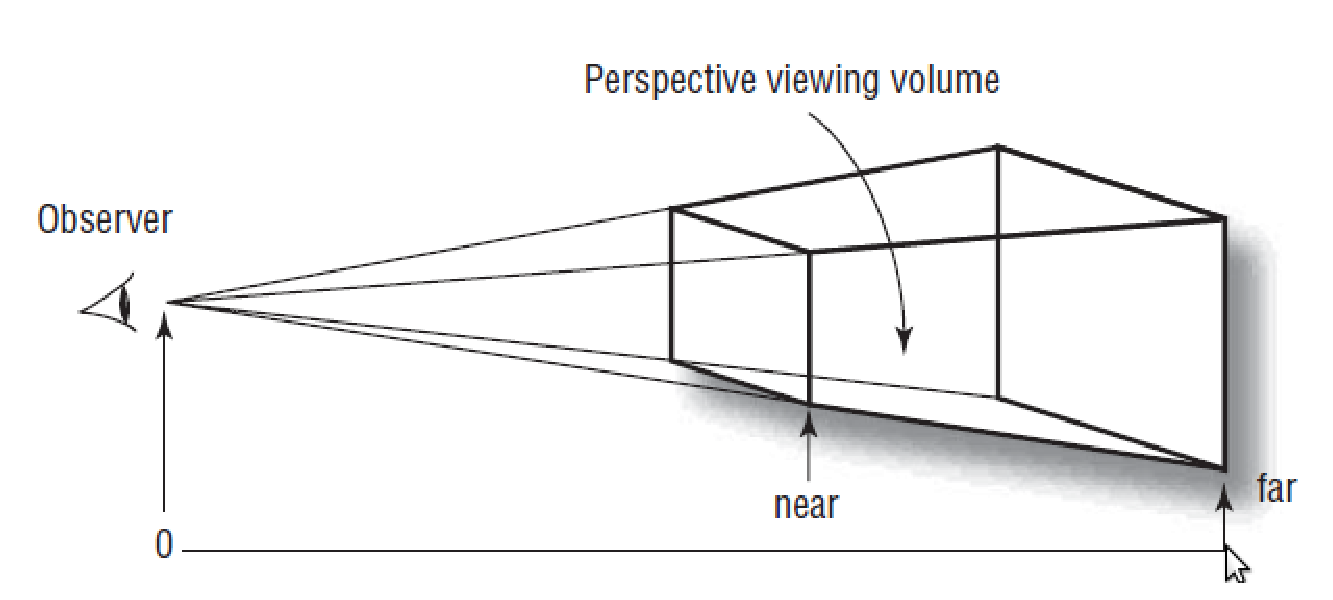
\includegraphics[height=4.5cm,
    angle=0]{./images/perspective_projection_2.eps}}
  \centerline{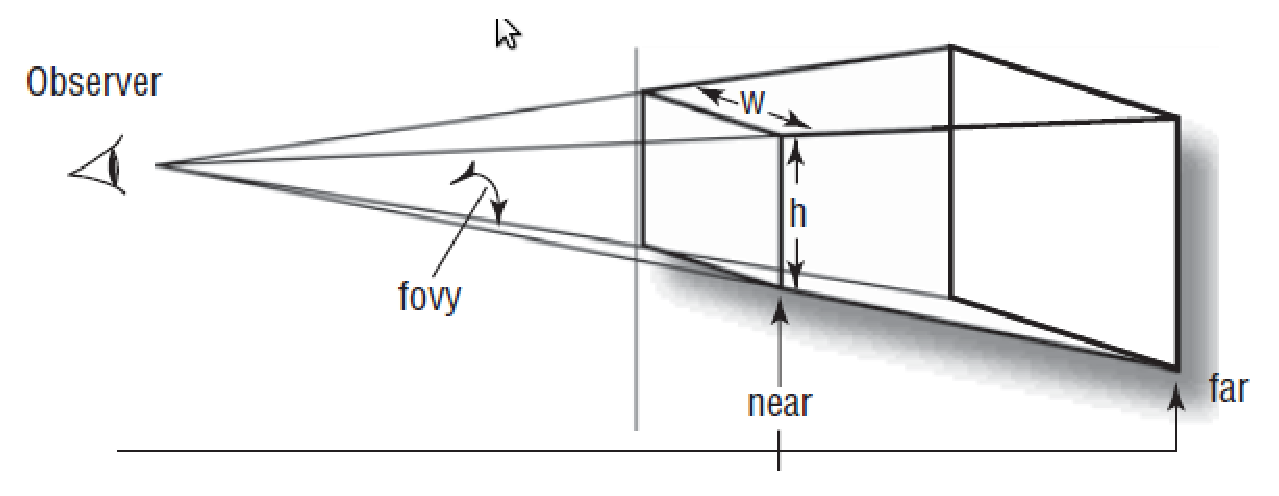
\includegraphics[height=3.8cm,
    angle=0]{./images/perspective_projection_3.eps}}
\caption{Perspective view}
\label{fig:perspective_2}
\end{figure}1

{\bf The question is how do we know what we plot fall inside this
  frustum?}. For example:
\begin{verbatim}
glBegin( GL_TRIANGLES );
glVertex2f( -0.5f, -0.5f, -10.0 );
glVertex2f( 0.5f, -0.5f, -10.0 );
glVertex2f( 0.0f, 0.5f, -10.0 );
glEnd();
\end{verbatim}
{\bf Frustum culling} is the technique that we need. There is no
OpenGL API or GLUT API to do this. However, it can be easily
implemented by
yourself\footnote{\url{http://www.opengl.org/resources/faq/technical/clipping.htm}}. 
\begin{enumerate}
\item We use a bounding sphere or cubeoid that just encloses all of
  the objects' vertices. This is called a 'bounding volume'.
\item And the question now is ``How do I tell if an arbitary sphere is
  either inside or crossing the six planes of the
  frustum?''\footnote{\url{http://www.sjbaker.org/steve/omniv/frustcull.html}} 
\end{enumerate}

\begin{framed}
  This describe frustum culling using cubeoid
  \begin{enumerate}
  \item Check if the z is more than the far plane value. If yes it can't
    be rendered. For eg:- if far = 50, anything with z < -50 ie z=-51
    and more will not be rendered

  \item Check if the z is less than near plane value. For eg:- near = 1,
    then anything above -1 will not render. So if z = 0 or z > 0 its
    outside the viewing volume

  \item Create a plane equation for left quad. Check if the triangle is
    inside the plane or not.

  \item Create a plane equation for right quad. Check if the triangle is
    inside or outside the plane.  Same goes for top and bottom.
  \end{enumerate}
\end{framed}


The question is when to use \verb!glOrtho!? It is typically used in
CAD application or for 2D graphics (e.g. 2D maps and onscreen head-up
displays).


Everything else needs to be done with the modelview matrix!

OpenGL has no notion of a "camera matrix" or world coordinate system.
The transformation after the modelview (i.e. model-to-view) coordinate
transformation has been applied your eye is in the origin of that
coordinate system (alas that's called eye-coordinate system).

To move your player forward you just transform the whole world in the opposite direction. Same for rotation of your player rotates to the left, just rotate the whole world to the right.

The only thing you need to consider for that is that the model- and
eye-coordinates are right handed in OpenGL Moving the player forward
means moving the world in +z-axis direction and so on...

\begin{verbatim}
//rendering a scene:
glMatrixMode(GL_PROJECTION);
glLoadIdentity();
glFrustum(...);
glMatrixMode(GL_MODELVIEW);
glLoadIdentity();
glRotatef(-cameraRoll, 0, 0, 1);
glRotatef(-cameraPitch, 1, 0, 0);
glRotatef(-cameraHeading, 0, 1, 0);
glTranslatef(-cameraPosition.x, -cameraPosition.y, -cameraPosition.z);

RenderWorld();   //static world

//repeat this for any movable object in the scene
glPushMatrix();
glTranslatef(objectPosision.x, objectPosision.y, objectPosision.z);
glRotatef(objectHeading, 0, 1, 0);
glRotatef(objectPitch, 1, 0, 0);
glRotatef(objectRoll, 0, 0, 1);
DrawObject();   //movable object
glPopMatrix();

\end{verbatim}

\begin{verbatim}
GLFrustum::SetOrthographic(GLfloat xMin, GLfloat xMax, GLfloat yMin,
            GLfloat yMax, GLfloat zMin, GLfloat zMax);

GLFrustum::SetPerspective(float fFov, float fAspect, 
                   float fNear, float fFar);
\end{verbatim}


\subsection{Off-screen rendering}
\label{sec:screen-rendering}

In the GPU pipeline, the traditional end point of every rendering
operation is the {\bf frame buffer}, a special chunk of graphics
memory from which the image that appears on the display is
read. Depending on the display settings (16bits, 24bits, or 32bits),
the most we can get is 32 bits of color depth, shared among the red,
green, blue and alpha channels of your display: Eight bits to
represent the amount of "red" in a image (same for green etc.: RGBA)
is all we can expect and in fact need on the display. Such
combinations already sums up to more than 16 million different
colors. 

Since we want to work with floating point values, 8 bits is clearly
insufficient with respect to precision. Another problem is that the
data will always be clamped to the range of [0/255; 255/255] once it
reaches the framebuffer. So, to create high-quality images, there is a
buffer - called {\bf offscreen buffer} which is an OpenGL extension
\verb!EXT_framebuffer_object! (aka {\bf FBO}) - that can be used as
the target of the rendering operations, providing full precision and
avoiding unwanted clamping issues.

\begin{framed}
  Why we need off-screen rendering?
  \begin{enumerate}
  \item generate intermediate images1 such as textures
  \item batch rendering of non-interactive animations
  \item high-resolution image generation for hard-copy, e.g. tiled
    rendering is a technique in which a large image is produced by
    tiling together smaller, individually rendered images. It's useful
    for generating images which are larger than what OpenGL would
    normally permit.
  \end{enumerate}
\end{framed}

Generally, off-screen rendering is not a core part of OpenGL. They are
provided as an extension such as GLX or
WGL\footnote{\url{http://www.mesa3d.org/brianp/sig97/offscrn.htm}}.  
\begin{enumerate}
\item Mesa provide OSMesa : off-screen rendering interfaces
\end{enumerate}

To use this extension and to turn off the traditional framebuffer and
use an offscreen buffer (surface) for our calculations, a few lines of
code suffice. 
\begin{verbatim}
GLuint fb;

void initFBO(void) {
    // create FBO (off-screen framebuffer)
    glGenFramebuffersEXT(1, &fb);
    // bind offscreen buffer
    glBindFramebufferEXT(GL_FRAMEBUFFER_EXT, fb);
}
\end{verbatim}


\begin{framed}
  Note that binding FBO number 0 will restore the window-system
  specific framebuffer at any time. This is useful for advanced
  applications but beyond the scope of this tutorial.
\end{framed}

Using FrameBuffer Object (FBO) is preferable for off-screen
rendering. For best performance, alternate rendering between two
different FBOs:
\begin{enumerate}
\item Render to A
\item Render to B
\item Read back from A and process it
\item Render to A
\item Read back from B
\item Goto 2
\end{enumerate}

Compared between rendering to a RenderBuffer vs. a Texture, rendering
to a renderbuffer is preferable. 


\section{Buffer objects (VBO vs. PBO vs. FBO)}
\label{sec:buffer-objects}

% \section{}
% \label{sec:vbo-vs.-pbo}

The power of graphics cards has been improved that can render meshes
with around 10 million vertices which requires hundreds of MB. The
main bottle neck now is the data bus for transmitting data from CPU
RAM to graphics card memory when processing data at this size, and the
transferring rate is high, e.g.  \verb!~!60 times per second across
the graphics bus. Traditional methods described in
Sect.~\ref{sec:interm-mode-vs} are no longer a good choice.


Besides drawing points, lines, polygons... (as shown in
Sect.~\ref{sec:interm-mode-vs}), in sect.~\ref{sec:arrays-=-textures},
we have learnt using texture to load image data for rendering. In this
section, we introduce a new technique to render and moving your data
around, as well as off-screen rendering. This can be done using
{\bf buffer objects}, and the data now can completely reside in
graphics memory.

Before OpenGL 3.2, you need to create hundreds of objects of varying
types. Now, we don't create geometric objects, we create buffer
objects. These buffer objects don't fix to a particular type of data,
i.e. it can reference to/hold vertex data, pixel data, texture data,
inputs for shader execution, or the output of different shader stages.

Create a new buffer object is simple, you can create a single or an
array of continuous buffer objects
\begin{verbatim}
!Fortran binding
INTERFACE
    SUBROUTINE glGenBuffers(n, buffers) BIND(C, name="glGenBuffers")
      USE iso_c_binding
      USE opengl_kinds
      INTEGER(Glsizei), VALUE:: n
      INTEGER(GLuint), DIMENSION(*) :: buffers
    END SUBROUTINE glGenBuffers

    SUBROUTINE glBindBuffer(n, buffer) BIND(C, name="glBindBuffer")
      USE iso_c_binding
      USE opengl_kinds
      INTEGER(GLenum), VALUE:: n
      INTEGER(GLuint), VALUE :: buffer
    END SUBROUTINE glBindBuffer
END INTERFACE
\end{verbatim}

\begin{verbatim}
Gluint pixBuffObjs[1];

glGenBuffers(1, pixBuffObjs);
\end{verbatim}
This will return you an integer value (the ID) - the name to the
buffer object. Each named buffer object can bind to a single target
and only one at a time. The target is known as the binding point, and
there are different types of them, as shown in
Table~\ref{tab:binding_point}. Each one serves a different purpose (to
be discussed shortly). 
\begin{verbatim}
glBindBuffer(GL_PIXEL_PACK_BUFFER, pixBuffObjs[0]);
\end{verbatim}

\begin{table}[hbt]
\begin{center}
\caption{Buffer object binding point}
\begin{tabular}{cp{7cm}} 
\hline
Target Name Description \\

\verb!GL_ARRAY_BUFFER! & Array buffers store vertex attributes such as color, position, texture
coordinates, or other custom attributes. \\
\verb!GL_COPY_READ_BUFFER! & Buffer used as the data source for copies with
glCopyBufferSubData. \\
\verb!GL_COPY_WRITE_BUFFER! & Buffer used as the target for copies
with glCopyBufferSubData. \\
\verb!GL_ELEMENT_ARRAY_BUFFER! & Index array buffer used for sourcing indices for glDrawElements,
glDrawRangeElements, and glDrawElementsInstanced. \\
\verb!GL_PIXEL_PACK_BUFFER! & Target buffer for pixel pack operations
such as glReadPixels. \\
\verb!GL_PIXEL_UNPACK_BUFFER! & Source buffer for texture update functions such as glTexImage1D,
glTexImage2D, glTexImage3D, glTexSubImage1D,
glTexSubImage2D, and glTexSubImage3D. \\
\verb!GL_TEXTURE_BUFFER! & Buffer accessible to shaders through texel
fetches. \\
\verb!GL_TRANSFORM_FEEDBACK_BUFFER! & Buffer written to by a transform
feedback vertex shader. \\
\verb!GL_UNIFORM_BUFFER! & Uniform values accessible to shaders. \\
\hline\hline
\end{tabular}
\end{center}
\label{tab:binding_point}
\end{table}


After binding a named buffer to target, we need to fill valid data
into it (i.e. filling the buffer)
\begin{verbatim}
// named buffer must be bound before calling this
glBufferData(GL_PIXEL_PACK_BUFFER, pixelDataSize, pixelData,
              GL_DYNAMIC_COPY);

\end{verbatim}

\begin{enumerate}
\item Pixel buffer objects are a great container for temporarily
  storing pixel data locally on the GPU, but remember they need to
  have storage allocated before they can be
  used.(Sect.~\ref{sec:pbo}). 

\item Just like all other buffer objects, calling \verb!glBufferData!
  allocates storage for a buffer and fills it with your data. But you
  don't necessarily have to provide data; passing in NULL for the data
  pointer simply allocates the memory without filling it.

\item If you don't allocate storage for a buffer before trying to fill
  it, OpenGL throws an error.
\end{enumerate}

\begin{framed}
  Note that this pointer to the third argument of
  \verb!glBufferData()! can also be NULL if you want to allocate a
  buffer of a specific size but do not need to fill it right away. The
  fourth parameter of \verb!glBufferData()! is where you tell OpenGL
  how you intend to use the buffer.
\end{framed}


Using \verb!GL_DYNAMIC_DRAW! is a safe value for general buffer usage
or situations where you aren't sure what the buffer will be used for
(read more later).  With that, you can always call \verb!glBufferData!
again, refilling the buffer and possibly changing the usage
hint. Recalling glBufferData, however, wipe out all data, to update
the new one. If only a small fraction of the data change, you can
improve the performance by telling OpenGL with
\verb!glBufferSubData()! to update a part of a preexisting buffer
without invalidating the contents of the rest of the buffer.

\begin{verbatim}
void glBufferSubData(GLenum target, intptr offset, 
                     sizeiptr size, const void *data);
\end{verbatim}
The \verb!offset! tell the offset (in bytes) from the beginning of the
buffer from which the update start. However, using
\verb!glBufferSubData()!, we cannot change the usage of the buffer,
e.g. change from \verb!GL_DYNAMIC_DRAW! to some thing else. 

When you are finished with a buffer, it needs to be cleaned up, just
as all other OpenGL objects should be. First, you need to unbind the
buffer, before you can delete the buffer.
\begin{verbatim}
// unbind the buffer: use the same binding point, with 
// the second argument is ``0'' 
glBindBuffer(GL_PIXEL_PACK_BUFFER, 0);

// make sure you unbound the buffer before delete it
glDeleteBuffers(1, pixBuffObjs);
\end{verbatim}
The unbound buffer can later bind to any other binding point. 



{\bf SUMMARY}: 
\begin{verbatim}
 // generate a VBO object
id = glGenBuffers(1)
 // tell what kind of data that VBO object
 // will reference to
glBindBuffer(target, id)

 // put the data to the buffer, along with tell how
 // often the data is modified
glBufferData(target, size, data, usage)
\end{verbatim}
with \verb!target! is one of those given in Table
\ref{tab:binding_point}., \verb!size! is the number of bytes to
transfer. \verb!data! is the big array containing the source data.

The \verb!usage! tell how often the data is updated/modified. There
are 3 modes of usage, with total 9 transfer modes (the first three
modes to support are \verb!GL_..._DRAW!)

\begin{itemize}
\item STATIC = specify the data only once, and use it many times
  without modifying it
  \begin{itemize}
  \item \verb!GL_STATIC_READ!
  \item \verb!GL_STATIC_COPY!
  \item \verb!GL_STATIC_DRAW! when vertex data never or almost never
    updated)
  \end{itemize}

  Data are sent only once from the CPU to the graphics card where they
  are saved in the graphic controller memory
  (\textcolor{red}{so it provides the highest performance}). This mode
  is suitable for non-deformable objects which remains unchanged
  during several frames

\item STREAM = modify the data once, then use it once, and repeat the
  process many time
  \begin{itemize}
  \item \verb!GL_STREAM_READ! 
  \item \verb!GL_STREAM_COPY!
  \item \verb!GL_STREAM_DRAW! when vertex data could be updated
    between each rendering)
  \end{itemize}

  This mode is particularly useful for CPU animated objects, i.e. data
  are sent each call to glDrawArrays, glDrawElements,
  glDrawRangeElements (\verb!EXT_draw_range_elements!, OpenGL 1.2)
  glMultiDrawArrays or glMultiDrawElements
  (\verb!EXT_multi_draw_array!, OpenGL 1.4).


\item DYNAMIC = specify/modify the data repeatedly, and use it
  repeatedly. 
  \begin{itemize}
  \item \verb!GL_DYNAMIC_READ! 
  \item \verb!GL_DYNAMIC_COPY!
  \item \verb!GL_DYNAMIC_DRAW! when vertex data could be updated
    between each frames
  \end{itemize}
  
  In this mode, the graphics driver will in charge of choosing the
  data location.
  \textcolor{red}{This mode is recommended for animated object that
    require rendering several time per frame}
\end{itemize}


\begin{framed}
  Mode \verb!GL_*_DRAW! provides the same behavior as Vertex Arrays
  (but used with glDrawArrays, glDrawElements, glDrawRangeElements,
  glMultiDrawArrays or glMultiDrawElements)

  Mode \verb!GL_..._READ!  allows you to read data managed by OpenGL.

  Mode \verb!GL_*_COPY!  allow displaying geometric from source
  managed by OpenGL.
\end{framed}
% With VBO, the OpenGL APIs tell the card to use the stored data instead
% of client-side vertex-sets when we want to render our geometry using
% array-based operations. This is the same basic operation we've done
% with textures and display lists. We store the data on the card
% identified by a unique ID for later reference and trigger its use when
% we would normally re-transfer the data.

% You can delete a single VBO or multiple VBOs with glDeleteBuffer(s) if
% they are not used anymore. After a buffer object is deleted, its
% contents will be lost.


\begin{framed}
  \verb!glMapBuffer! is synchronous mapping.  To avoid waiting (idle),
  you can call first glBufferDataNull, then call glMapBuffer. In this
  case, the previous data will be discarded and glMapBuffer returns a
  new allocated pointer immediately even if GPU is still working with
  the previous data.

  However, this method is valid only if you want to update entire data
  set because you discard the previous data. If you want to change
  only portion of data or to read data, you better not release the
  previous data.

\end{framed}


\subsection{VBO}
\label{sec:vbo}

Vertex buffer object (VBO) is an extension in OpenGL 1.4 and become
the standard in OpenGL
1.5\footnote{ VBOs are also available with OpenGL ES 2.0 but this
  feature is optional.}.
So, all OpenGL APIs working with VBO in OpenGL 1.4 should be prefixed
with \verb!ARB!, e.g. \verb!glGenBuffersARB()!.
\textcolor{red}{``Features, efficiency and longevity are three reasons
  to use VBOs as soon as possible''}.

VBO are buffers into which we can load vertex array data
(Sect.~\ref{sec:vertex-arrays}), as well as color, normal, and face
indexing data. These data can reside in high-performance graphics
memory, i.e. the server side, and thus promotes efficient data
transfer. 
\begin{itemize}
\item Color, normal and coordinate arrays are passed as 'just array
  buffers' \verb!GL_ARRAY_BUFFER!, and use glColorPointer(),
  glVertexPointer(), glNormalPointer() for rendering.

\item Indexed faces are passed using element array buffers
  \verb!GL_ELEMENT_ARRAY_BUFFER!, and use glDrawElements() for rendering.
\end{itemize}

\begin{framed}
  VBO (Vertex Buffer Objects (Arrays)) is a techniques that OpenGL use
  to connect to geometry (vertex) data that reside in ``fast'' memory
  (i.e. video RAM). Though we can associate the data with a VBO
  object, the actual storage location of the data is hidden from you.

  VBO are similar in principles to PBO but provide lots of
  improvements with 3 transfer modes (i.e. access pattern) compared to
  using PBO. We use VBO to generate 3D meshes and utilize OpenGL VBOs
  (Vertex Buffer Objects) to efficiently render meshes as a colored
  surface, wireframe image or set of 3D points.

% \begin{verbatim}
% glGenBuffersARB
% glBindBufferARB
% glDeleteBufferARB
% ..
% ..
% (and so on)
% \end{verbatim}
\end{framed}

% VBO code looks pretty much like regular OpenGL 1.1 array-using
% code. You build the same arrays, but instead of passing the arrays
% into OpenGL, you set up a VBO object and load the data into it. A VBO
% object is simply an integer or an array of integers that we use to get
% reference to data residing on the server side (i.e. graphics card
% memory).
\textcolor{red}{Creating a VBO requires these functions}:

\begin{itemize}
\item \verb!glGenBuffers()!: create one or a continuous array of VBOs
  (handle variable)
\begin{verbatim}
GLvoid glGenBuffers(GLsizei n, GLuint* buffers);
\end{verbatim}
  with $n$ is the number of VBO objects, $buffers$ is an integer array
  (or a scalar) keeping the VBO objects' IDs.  

\item \verb!glBindBuffer()!: active the buffer (or make the handle
  ``current''). Here, instead of addressing the memory using pointer,
  we address buffers using handle. This buffer will later be loaded
  with data

\item\verb!glBufferData()!, or \verb!glBufferSubData()!: copy
  vertex/color/normal/ data to the buffer: which are conceptually
  similar to \verb!glTexImage*()! and \verb!glTexSubImage*()!.
  \begin{itemize}
  \item call \verb!glBufferData()! to get a pointer to the VBO (with
    desired mode: \verb!GL_READ_ONLY, GL_WRITE_ONLY, GL_READ_WRITE!),
    then write data to it, and finish by calling
    \verb!glUnmapBuffer()!

  \end{itemize}

\item \verb!glDeleteBuffers()!: delete the buffer
\begin{verbatim}
GLvoid glDeleteBuffers(GLsizei n, const GLuint* buffers);
\end{verbatim}

\end{itemize}
If you use \verb!glBufferDataNull! instead, then no data parameter is
provided and then VBO reserves only memory space with the given data
size. 

{\bf Example}:
\begin{enumerate}
\item Call this code (or similar) ONCE (i.e. not inside the callback)
  for each array you want to buffer
\begin{verbatim}
// this example illustrates how to load a vertex array buffer.
// only small variations for loading color arrays
// and element (indexed triangle) arrays.
// see the rest of the article for details.
// create a handle that you will use to refer to the buffer when talking to gl
GLuint handle;
glGenBuffers(1,&handle);
// let's load our buffer data...
// size of your buffer, here, 3 times the number of vertices,
// multiplied by your format size, for example sizeof(GL_FLOAT).
int dataByteSize = ...
float* data = malloc(dataByteSize)
// need to populate your buffer with vertex data!
...
// this loads 'data' into graphic memory referred by 'handle'
glBindBuffer(GL_ARRAY_BUFFER,handle);
// Typically you want to use static draw. This implies you will use the buffer
// over and over, in other words you won't modify geometry afterwards.
glBufferData( GL_ARRAY_BUFFER, dataSize, data, GL_STATIC_DRAW);
// clear the binding after loading your array, otherwise you will get crashes
glBindBuffer(GL_ARRAY_BUFFER,0);
\end{verbatim}

\item Put this inside the callback (rendering)
\begin{verbatim}
// this example illustrates how to 'pass pointers' with
// 'pass array buffers'
// note: this example only makes sense if you can do basic gl rendering.
glBindBuffer(GL_ARRAY_BUFFER,handleToColorBuffer);
glVertexPointer(4,GL_FLOAT,0,0 /*replaced the pointer reference by zero*/ );
glBindBuffer(GL_ELEMENT_ARRAY_BUFFER,handleToPerFaceVertexIndices);
glDrawElements(... , 0 /*replaced the pointer reference by zero*/ );
\end{verbatim}

\end{enumerate}

{\bf Example}: draw a cube
\begin{enumerate}
\item Allocate the new buffer
\begin{verbatim}
// allocate a new buffer
glGenBuffers(1, &cubeVBO);
// bind the buffer object to use
glBindBuffer(GL_ARRAY_BUFFER, cubeVBO);
\end{verbatim}

\item Normally, the data involve vertex and color information. 
\begin{verbatim}
const GLsizeiptr vertex_size = NUMBER_OF_CUBE_VERTICES * &
       NUMBER_OF_CUBE_COMPONENTS_PER_VERTEX*sizeof(GLfloat);
const GLsizeiptr color_size = NUMBER_OF_CUBE_COLORS * &
       NUMBER_OF_CUBE_COMPONENTS_PER_COLOR*sizeof(GLubyte);
\end{verbatim}

\item Copy the data to the VBO object, and tell how often we want to
  modify the data (this will help OpenGL works  better)
\begin{verbatim}
// allocate enough space for the VBO
glBufferData(GL_ARRAY_BUFFER, vertex_size+color_size, 0, GL_STATIC_DRAW);
\end{verbatim}
  We have two different pieces of data, the vertices and the
  colors. For this case, \verb!glBufferSubData! is one way of copying
  sections of data into the buffer. Another way is to use
  \verb!glMapBuffer!. At a high level, glMapBuffer is sort of like
  direct memory access (DMA) for your video card. It potentially
  avoids an extra system copy by creating a direct map of memory.

  For example, we use glMapBuffer
\begin{verbatim}
GLvoid* vbo_buffer = glMapBuffer(GL_ARRAY_BUFFER, GL_WRITE_ONLY_OES);
	// transfer the vertex data to the VBO
	memcpy(vbo_buffer, s_cubeVertices, vertex_size);

	// append color data to vertex data. To be optimal,
	// data should probably be interleaved and not appended
	vbo_buffer += vertex_size;
	memcpy(vbo_buffer, s_cubeColors, color_size);
glUnmapBuffer(GL_ARRAY_BUFFER); 
\end{verbatim}
  As you can see, color information cluster at one place, vertex
  information cluster at another place. This makes the copying
  straightforward, though is not recommended, as OpenGL prefer
  interleaved data, i.e. vertex data, color data, vertex data, color
  data... This will allow drawing a single point faster as it can
  easily and quickly obtain the location and color information of that
  point. This is particularly important if we have more information
  \textcolor{red}{(position, color, texture coordinates, normals)}.

\item After the VBO object has referenced/mapped to the data, we need
  to tell how the data is organized (as in the beginning OpenGL only
  know this is a chunk of byte)
\begin{verbatim}
// Describe to OpenGL where the vertex data is in the buffer
/* we tell OpenGL we have vertices with 
       - 3 components per vertex (x, y, x) 
       - and they are GL_FLOATs. 
       - stride = 0
       - starting from the beginning of the array. 
*/
glVertexPointer(3, GL_FLOAT, 0, (GLvoid*)((char*)NULL));

// Describe to OpenGL where the color data is in the buffer
/* For the color data where we have 
       - 4 components (R, G, B, A)
       - each is GL_UNSIGNED_BYTEs
       - stride = 0
       - and start in the array position after the vertex points.
*/
glColorPointer(4, GL_UNSIGNED_BYTE, 0, & 
              (GLvoid*)((char*)NULL+vertex_size));
\end{verbatim}
  If you have texture coordinates or normals, don't forget to use
  glTexCoordPointer and glNormalPointer in the same
  way. \textcolor{red}{The order of calling these functions are
    important}. 

\item Now, we still need an index array (some people call this Index
  Buffer Objects (IBOs)) and now we use \verb!GL_ELEMENT_ARRAY_BUFFER!
  instead of \verb!GL_ARRAY_BUFFER! in our call to glBindBuffer. This
  is what distinguishes the IBO from the VBO.
\begin{verbatim}
// create index buffer
glGenBuffers(1, &cubeIBO);
glBindBuffer(GL_ELEMENT_ARRAY_BUFFER, cubeIBO);

/* For constrast, instead of glBufferSubData and glMapBuffer,
   we can directly supply the data in one-shot, i.e. pass the
   data when you first allocate the memory. We can do this as
   we don't need to combine separate arrays (like for vertex 
   and color)
*/
glBufferData(GL_ELEMENT_ARRAY_BUFFER, & 
     NUMBER_OF_CUBE_INDICES*sizeof(GLubyte), & 
     s_cubeIndices, GL_STATIC_DRAW);
\end{verbatim}

\item At this point, we can render
\begin{verbatim}
// Activate the VBOs to draw
glBindBuffer(GL_ARRAY_BUFFER, cubeVBO);
glBindBuffer(GL_ELEMENT_ARRAY_BUFFER, cubeIBO);

glEnableClientState(GL_VERTEX_ARRAY);
glEnableClientState(GL_COLOR_ARRAY);

/* This is the actual draw command
  Without it, nothing will be drawn.
*/
glDrawElements(GL_TRIANGLE_STRIP, NUMBER_OF_CUBE_INDICES, &
       GL_UNSIGNED_BYTE, (GLvoid*)((char*)NULL));
\end{verbatim}
  We bind the buffers. We tell the system we want to draw vertices and
  colors. (We don't have normals and texture coordinates in this
  example, but if we did we would also need to enable
  \verb!GL_NORMAL_ARRAY! and \verb!GL_TEXTURE_COORD_ARRAY!.)

\item Before we exit, we need to clean up the resource
\begin{verbatim}
glDeleteBuffers(1, &cubeIBO);
glDeleteBuffers(1, &cubeVBO);
\end{verbatim}
\end{enumerate}
\url{http://playcontrol.net/ewing/jibberjabber/opengl_vertex_buffer_object.html} 


VBO are unformatted objects, i.e. they are a big chunk of bytes. Thus,
OpenGL doesn't care whether they contain float data, what the ordering
is ... until you call a ``draw'' function. Rendering a VBO is almost
similar to rendering the array. Therefore, no additional APIs are
required to draw VBO except glBindBuffer.
\begin{verbatim}
// bind VBOs for vertex array and index array
glBindBuffer (GL_ARRAY_BUFFER, vboId1);//  (* for vertex coordinates *)
glBindBuffer (GL_ELEMENT_ARRAY_BUFFER, vboId2);// (* for indices *)

//(* do same as vertex array except pointer *)
glEnableClientState (GL_VERTEX_ARRAY);//(* activate vertex coords array *)
glVertexPointer(3, GL_FLOAT, 0, 0); // (* last param is offset, not ptr *)

//(* draw 6 quads using offset of index array *)
glDrawElements GL_QUADS 24 GL_UNSIGNED_BYTE 0;

glDisableClientState GL_VERTEX_ARRAY;  //(* deactivate vertex array *)

(* unbind, so switch back to normal pointer operation *)
glUnbindBuffer GL_ARRAY_BUFFER;
glUnbindBuffer GL_ELEMENT_ARRAY_BUFFER;
\end{verbatim}

% Like glBufferData, glBufferSubData is used to copy data into VBO, but
% it only replaces a range of data into the existing buffer, starting
% from the given offset. (The total size of the buffer must be set by
% glBufferData before using glBufferSubData.)  


We can update VBO data (which can not be done with
{\bf display list}).
\begin{enumerate}
\item the simplest way: copy new data into the bound VBO with
  glBufferData or glBufferSubData. Here, we need 2 copies of vertex
  data: one in your application and one in your VBO, then we can
  switch between them. 

\item
  \textcolor{red}{ The second improvement that characterise VBO sis
    called Vertex mapping (see CUDA-OpenGL)}.  Instead of telling
  OpenGL to copy the data into the VBO buffer, we can tell it to
  temporarily map buffer object into client's memory, then the
  client can update the data with a pointer to the mapped buffer
  using \verb!glMapBuffer!. This is similar to that being used in
  CUDA-OpenGL interop, when we map buffer object to CUDA memory
  space.
\begin{verbatim}
glMapBuffer(target, access, ...)
\end{verbatim}
  with access can be
\begin{verbatim}
GL_READ_ONLY
GL_WRITE_ONLY
GL_READ_WRITE
\end{verbatim}

  After that, unmapped the data from client's memory, to avoid it being
  modified by any other process.
\end{enumerate}


VBOs provide an excellent alternative to interleaved arrays. As a
recalling, interleaved arrays allow sending vertices data to the
graphics card using a single array decribes by the function
\verb!glInterleavedArrays!. With vertex arrays, we must using
predefined data structures with defined order for each element of this
structure. With GPU programming arising, programmer custom attributes
aren't managed by this solution. VBOs solve this issue and allow
updated of only a part of the data.


\subsection{PBO}
\label{sec:pbo}

{\bf Pixel Buffer Objects} (PBO) is not new. Pixel buffer objects are
similar to texture buffer objects in that they hold pixel/texel data;
yet the data now reside on GPU.

Possible binding targets for PBO are
\begin{verbatim}
GL_PIXEL_PACK_BUFFER
    When a PBO is attached to this target, 
    any OpenGL operations that "read" pixels get their data from the PBO
 -> glReadPixels, glGetTexImage, and glGetCompressedTexImage
  
GL_PIXEL_UNPACK_BUFFER
    any OpenGL operations that "draw" pixels put their data 
    into an attached PBO.
 -> glTexImage*D, glTexSubImage*D, glCompressedTexImage*D,
      and glCompressedTexSubImage*D.


\end{verbatim}

All calls to \verb!glBufferData()! are pipelined with the rest of your
draw calls. That means the OpenGL implementation won't have to wait
for all activities to stop before sending the new data to the GPU.

\begin{framed}
  Pixel buffers are often used to hold 2D images coming from a
  renderbuffer target, texture, or other source.
  \textcolor{red}{However, buffer objects are one-dimensional by
    nature; they don't have an intrinsic width or height}.
  When allocating storage space for 2D images, you can just multiply
  the width by the height by the size of a pixel.

    If you plan to use the same PBO for multiple data sizes, you are
    much better off sizing the PBO for the largest data set right away
    than resizing it frequently.
\end{framed}

We use PBO to create images with CUDA on a pixel-by-pixel basis and
display them using OpenGL. PBO (Pixel Buffer Objects) is not a new
OpenGL object (added to OpenGL 2.1). It just says ``we can use the
buffer object for pixel operations, not just geometry operations''.


After you render the frame, i.e. the data is sent to renderbuffer, you
may want to read the data \textcolor{red}{ back to client memory},
e.g. use the data from previous frames to apply the effect on the next
frame. To do so, we use \verb!glReadPixels()! (to read back to GPU
memory, read the solution later)
\begin{verbatim}
void* data = (void*)malloc(pixelDataSize);
glReadBuffer(GL_BACK_LEFT);
glReadPixels(0, 0, GetWidth(), GetHeight(), GL_RGB, GL_UNSIGNED_BYTE, pixelData);
\end{verbatim}
Before reading back to client memory, the entire pipeline often has to
be emptied to ensure all drawing that would affect the pixels you are
about to read has completed.  This can have a major impact on your
application's performance. But the good news is we can use buffer
objects to overcome this performance issue. You can bind a buffer
object to the \verb!GL_PIXEL_PACK_BUFFER! before you call glReadPixels
and set the data pointer in the glReadPixels call to null. This
redirects the pixels into a buffer located on the GPU and avoids the
performance issues that copying to client memory can cause.
\begin{verbatim}
glReadBuffer(GL_BACK_LEFT);
glBindBuffer(GL_PIXEL_PACK_BUFFER, pixBuffObjs[0]);
glReadPixels(0, 0, GetWidth(), GetHeight(), GL_RGB, GL_UNSIGNED_BYTE, NULL);
\end{verbatim}

\subsubsection{Blur effect}
\label{sec:blur-effect}

What we can do 
\begin{enumerate}
\item An application can render multiple times to a buffer, slightly
  offsetting the fast moving objects and blending the results
  together. 
\item Another option is to sample texel data for an object image
  multiple times in the direction of movement and then blend the
  sample results together. 
\item There are even more involved methods that use depth buffer data
  to apply a more dramatic blur to objects closer to the camera.  

\item A simple approach is stores the results of previous frames and
  blends them together with the current frame
\end{enumerate}

Simple approach: we use texture and PBO. Here, 6 textures units are
used for blur effect. Here, we dont use swap; the result is copied
into a texture to be used for the blur effect.
\begin{verbatim}
// Create blur textures
  glGenTextures(6, blurTextures);
// Allocate a pixel buffer to initialize textures and PBOs
  pixelDataSize = GetWidth()*GetHeight()*3*sizeof(unsigned byte);
  void* data = (void*)malloc(pixelDataSize);
  memset(data, 0x00, pixelDataSize);
// Setup 6 texture units for blur effect
// Initialize texture data
for (int i=0; i<6;i++)  {
  glActiveTexture(GL_TEXTURE1+i);
  glBindTexture(GL_TEXTURE_2D, blurTextures[i]);
  glTexParameteri(GL_TEXTURE_2D, GL_TEXTURE_WRAP_S, GL_CLAMP_TO_EDGE);
  glTexParameteri(GL_TEXTURE_2D, GL_TEXTURE_WRAP_T, GL_CLAMP_TO_EDGE);
  glTexParameteri(GL_TEXTURE_2D, GL_TEXTURE_MIN_FILTER, GL_LINEAR);
  glTexParameteri(GL_TEXTURE_2D, GL_TEXTURE_MAG_FILTER, GL_LINEAR);
  glTexImage2D(GL_TEXTURE_2D, 0, GL_RGB, GetWidth(), GetHeight(), 0, GL_RGB,
                 GL_UNSIGNED_BYTE, data);
}

// Allocate space for copying pixels so we don't call malloc on every draw
glGenBuffers(1, pixBuffObjs);
glBindBuffer(GL_PIXEL_PACK_BUFFER, pixBuffObjs[0]);
glBufferData(GL_PIXEL_PACK_BUFFER, pixelDataSize, pixelData, GL_DYNAMIC_COPY);
glBindBuffer(GL_PIXEL_PACK_BUFFER, 0);
\end{verbatim}
If texture 3 was used last time, texture 4 will be used next. That
means texture 4 will contain data from this frame, texture 3 from the
last, texture 2 from two frames ago, and so on.

The target for the current frame wraps around again after the last
texture has been used. The pixel data for the last six frames is
always ordered and available in this 'texture ring buffer'.For the
traditional path, this happens by calling glReadPixels to get the
pixel data and then glTexImage2D to move the pixel data into a texture
object.

\begin{framed}
  On slower systems the PBO path is almost six times faster than the
  client memory path.
\end{framed}
The PBO path is slightly different. Instead of copying the data back
to the CPU, the PBO is bound to the \verb!GL_PIXEL_PACK_BUFFER!, and
when we call glReadPixels, the pixels are redirected to the PBO
instead of back to the CPU. Then that same buffer is unbound from the
\verb!GL_PIXEL_PACK_BUFFER! attachment and bound to the
\verb!GL_PIXEL_UNPACK_BUFFER!. When glTexImage2D is called next, the
pixel data in the buffer is loaded into the texture, all without ever
leaving the GPU and remaining pipelined with other OpenGL commands.
You can see this process in Listing 8.2. Finally, the ring buffer is
updated to point to the next blur texture. You can press the P button
while running the program to switch between the two paths.

\subsection{TBO }
\label{sec:tbo-}

Texture Buffers allow you to do many things that traditional buffers
cannnot do. 

\subsection{FBO}
\label{sec:fbo}


Normally, rendering write out the graphics to a window or the full
screen. So, a default framebuffer object is created and bound to the
window automatically when an OpenGL context is created.  Now, OpenGL
give you the option to create multiple framebuffer objects (FBO) and
you can render to these FBO, instead to the framebuffer bound to the
window. This is known as {\bf off-screen rendering}
(Sect.~\ref{sec:screen-rendering}.

FBO is a new and better choice. It replaces previous render-to-texture
methods (e.g. offscreen window, PBuffers) (added to OpenGL 3.0). FBOs
are not limited to the size of the window and can contain multiple
color buffers, i.e. allow rendering high resolution output.
\begin{framed}
  Framebuffers are not really buffers, i.e. there is no real memory
  storage associated with a framebuffer object (FBO). Instead, FBOs
  are containers that can hold other objects that do have memory
  storage and can be rendered to, such as textures or renderbuffers. 

  So, before we can render to an FBO, we have to add images
\end{framed}


\begin{framed}
  MIP maps (or {\bf mipmaps}) are pre-calculated, optimized set of
  images (i.e. sequence of textures), each is a progressively lower
  resolution representation of the same image, that accompany a main
  texture that help increase the rendering speed and reduce
  antialiasing.

  Normally, the image in the main texture is of largest size
  (e.g. 256x256), and the images in the mipmaps set is the smaller
  sizes (128x128, 64x64, 32x32, 16x16...).  By keeping multiple copies
  at different level of detail, the render can switch to the suitable
  mipmap image when the texture is viewed from a distance or at a
  smaller size.

  In some cases, we may want the images in the mipmaps set to be
  nonuniform compared to the main texture, known as {\bf ripmaps},
  e.g. 128x64, 128x32, ... However, ripmaps are unpopular due to
  higher memory demand. 
\end{framed}

When we draw, we often need an RGBA image buffer and a 32-bit depth
buffer that is separate (or may be there are other buffers too). FBO
allows drawing into RGBA texture and DEPTH-type buffers at the same
time.  

\subsection{Reading data from buffer objects}
\label{sec:reading-data-from}

The previous sections tell you how to load data into a target-bound
named buffer. Now, we will learn how to read the data back which may
be helpful in some cases.

We'll takes pixels from the currently enabled read buffer and copies
them into local CPU memory
\begin{verbatim}
void* data = (void*)malloc(pixelDataSize);
glReadBuffer(GL_BACK_LEFT);
glBindBuffer(GL_PIXEL_PACK_BUFFER, pixBuffObjs[0]);

glReadPixels(0, 0, GetWidth(), GetHeight(), 
            GL_RGB, GL_UNSIGNED_BYTE, pixelData);
\end{verbatim}


\section{OpenXX}
\label{sec:openxx}

There are many Open-standard being used nowadays
\begin{itemize}
\item OpenCL (Open Computing Language) = lower level of CUDA
\item OpenAL (Open Audio Library) = cross-platform audio APIs
\item OpenML (Open Media Library) = cross-platform programming
  environment for capturing, transporting, processing, displaying, and
  synchronizing digital media (2D/3D graphics, audio \& video, I/O,
  networking) 
\item OpenSL ES (Open Sound Library for Embedded Systems) = C-language
  audio API for 2D/3D audio being used in mobile and gaming industry. 
\end{itemize}

Read more on Chap.~\ref{chap:cuda-opengl}. 

\chapter{Mesa}
\label{chap:mesa}
\label{sec:mesa}


Mesa is a term used to encompass the different open source graphics drivers
available on Linux, so it can be what powers your GPU. 
Mesa itself is not a driver, as you will be using a different part of Mesa for
each graphics card vendor.  

Nowadays, we call it Mesa3D, it implements 3D graphics library
(Sect.\ref{sec:mesa-3d})

Originally, Mesa began only to serve as an open source Linux implementation of
OpenGL (Chap.\ref{chap:opengl}), but it has since grown to be a lot more than
that. Mesa implements various API's (Application programming interface) like
OpenGL, OpenGL ES, OpenCL, OpenMAX, VDPAU, VA API, XvMC and Vulkan.


Mesa was started in 1993 by Brian Paul (for freedesktop.org), but now it has
many more developers, some of which are employed by the likes of AMD, Intel,
Valve and others.
Linux game porters like Feral Interactive have also contributed code to Mesa.
Plenty of people also help with Mesa development in their spare time too.

\section{Mesa driver}

You may not using Mesa driver, depending upon the GPU device
\begin{enumerate}
  \item Intel HD Graphics card: you must be using Mesa

Exception: Intel usually supports Mesa quite well and even have their own Mesa
update tool named 'Intel Graphics Update Tool' to give certain distributions
the latest version of Mesa. 
 
  \item AMD GPU:   most AMD graphics cards have pretty good support in Mesa,
  with the closed source driver often not being needed.

The latest AMD cards use the \verb!amdgpu! kernel driver (the proprietary
AMDGPU-PRO also uses a version of this, which has not yet been accepted into the
Linux kernel yet), whereas all older cards use the \verb!radeon! kernel driver.
Each part of Mesa listed below hooks into one of those kernel drivers.

\begin{verbatim}
radeon - R100 series
r200 - R200 series
r300g - R300, R400, and R500 series
r600g - R600, R700, HD 5000 and HD 6000
radeonsi - HD 7000, HD 8000 and RX 200, RX 300 and RX 400

You also have the 'radv' driver for Vulkan, which was officially added in Mesa
13. It's still in development right now, so it's to be considered in beta.  
\end{verbatim}
  
  \item Nvidia GPUs: For NVIDIA, it's usually best to stick with the proprietary
  driver, ie. dont' use Mesa. 

 
  NVIDIA doesn't help towards development of Mesa, since they prefer their own
  closed-source proprietary drivers. For NVIDIA cards Mesa is typically quite
  far behind the closed drivers in terms of performance and features due to
  this. Mesa also typically doesn't work well, if at all with the very latest
  generation of NVIDIA graphics cards.   



With Mesa, you have the nouveau (pronounced like nu-vo) kernel driver, but like
AMD, NVIDIA uses nouveau plus another part of Mesa depending on your graphics
card model.

Later generations of NVIDIA cards require something called 'signed firmware' in
order for Mesa to interact with them and NVIDIA has been quite slow to release
it. The 'Pascal' generation in particular right now has very little support, as
NVIDIA has only recently provided the signed firmware required.
  
\end{enumerate}
\url{https://www.gamingonlinux.com/articles/an-explanation-of-what-mesa-is-and-what-graphics-cards-use-it.9244}

Versioning:
\begin{verbatim}
glxinfo | grep Mesa
\end{verbatim}

Get the latest {\it stable} Mesa driver for AMD and Intel
\begin{verbatim}
sudo add-apt-repository ppa:paulo-miguel-dias/pkppa
sudo apt-get update


\end{verbatim}

We need
\begin{verbatim}
Mesa 9.1.3
   GLproto 1.4.16
      util-macros-1.17 (ignore what 'make' tell you)
      libdrm-2.4.24+ (.36, .42)
      dri2proto-2.8 (modify configure.ac bloack XORG...)
  libxcb-1.9
      xcb-proto-1.8
  libtool-2.4.2
  pkg-config-0.27.1
  automake-1.12

Mesa 9.0.3
   GLproto 1.4.16
      util-macros-1.17 (ignore what 'make' tell you)
      libdrm-2.4.24+ (.36, .42)
      dri2proto-2.8 (modify configure.ac bloack XORG...)
  libxcb-1.9
      xcb-proto-1.8
  makedepend 1.0.3 
\end{verbatim}

Download links:
\begin{enumerate}
  \item automake (Sect.\ref{sec:automake}):
  

  \item
  pkg-config:\footnote{\url{http://people.freedesktop.org/~dbn/pkg-config-guide.html}}
  \url{http://pkgconfig.freedesktop.org/releases/}
  
  \item libtool: \url{http://mirror.rit.edu/gnu/gnu/libtool/}
  
  \item util-macro: \url{http://cgit.freedesktop.org/xorg/util/macros}
  We need to put in the ~/.bashrc file
\begin{verbatim}
alias cls='clear'
export PKG_CONFIG_PATH=$HOME/local/share/pkgconfig/:$PKG_CONFIG_PATH
export PKG_CONFIG_PATH=$PKG_CONFIG_PATH:$HOME/local/lib/pkgconfig/:/usr/share/pkgconfig/
export GLPROTO_CFLAGS=-I$HOME/local/include
export GLPROTO_LIBS=$HOME/local/lib/pkgconfig/
export XORG_MACROS_VERSION=1.17
export PATH=$HOME/local/bin:$PATH
export PKG_CONFIG_PATH=$PKG_CONFIG_PATH:$HOME/local/share/aclocal/
\end{verbatim}  

\item makedepend: 

  \end{enumerate}

Commands to use when we want to install into our home folder
\begin{verbatim}
./configure --prefix=/vlsci/VR0236/tmhoangt/local/ 2>&1 | tee c.txt
make -j4  2>&1 | tee m.txt
make install 2>&1 | tee mi.txt
\end{verbatim}
However, there are situations that we need to edit \verb!configure.ac!
explicitly.

When you \verb!make! some of the tools, it just say
\begin{verbatim}
make: Nothing to be done for `all'.
\end{verbatim}
we just ignore and continue with \verb!make all!.

\label{sec:xorgs-macro}
If xorgs-macro has not been installed, run
\begin{verbatim}
sudo apt-get install xutils-dev
\end{verbatim}

When you get the error about \verb!XORG_MACROS_VERSION!, it means it cannot
automatically find where \verb!xorg-macros.m4!
\begin{verbatim}
~/local/share/aclocal/xorg-macros.m4 
\end{verbatim}
So, you modify the \verb!configure.ac! file
\begin{verbatim}

///something here

# Require X.Org macros 1.8 or later for MAN_SUBSTS set by XORG_MANPAGE_SECTIONS
m4_ifndef([XORG_MACROS_VERSION],
          [m4_fatal([must install xorg-macros 1.8 or later before running autoconf/autogen])])
XORG_MACROS_VERSION(1.8)

///something here
\end{verbatim}
What you do is
\begin{enumerate}
  \item Remove the part after \verb!XORG_MACROS_VERSION(1.8)! and save to tmp
  file
  \item Remove the part below as well
\begin{verbatim}
# Require X.Org macros 1.8 or later for MAN_SUBSTS set by XORG_MANPAGE_SECTIONS
m4_ifndef([XORG_MACROS_VERSION],
          [m4_fatal([must install xorg-macros 1.8 or later before running autoconf/autogen])])
XORG_MACROS_VERSION(1.8)
\end{verbatim}  

  \item Concatenate the content of xorg-macros.m4 at the end of
  \verb!configure.ac! file
  \begin{verbatim}
cat ~/local/share/aclocal/xorg-macros.m4 >> configure.ac
  \end{verbatim}
  \item Concatenate the tmp file into configure.ac again
  \item Run ./autogen.sh to generate \verb!configure! file
  (Sect.\ref{sec:configure})
\end{enumerate}

When you get the error
\footnote{\url{http://stackoverflow.com/questions/10085554/libtool-version-mismatch}}
\begin{verbatim}
libtool: Version mismatch error.  This is libtool 2.4.2, but the
libtool: definition of this LT_INIT comes from an older release.
libtool: You should recreate aclocal.m4 with macros from libtool 2.4.2
libtool: and run autoconf again.
\end{verbatim}
then we run
\footnote{\url{http://www.openismus.com/documents/linux/building_libraries/building_libraries}}
\begin{verbatim}
autoreconf -fvi
\end{verbatim}
We expect \verb!bootstrap! method should work, but may be not for all the
cases\footnote{\url{http://www.sourceware.org/autobook/autobook/autobook_43.html}}.
Another suggestion is to run
\begin{verbatim}
$ vim configure.ac
$ libtoolize --force
$ aclocal
$ autoheader
$ automake --force-missing --add-missing
$ autoconf
\end{verbatim}
to create a functional \verb!configure!
file.\footnote{\url{https://bbs.archlinux.org/viewtopic.php?id=161452}}

\begin{framed}
Each platform has their own ways of building static or shared libraries.
\verb!libtool! provides automake and autoconf the unified option to build shared
libraries for  many operating systems using the same build files. 
If libtool is installed, then we can call \verb!LT_INIT! in the configure.ac
file. 
\end{framed}


\chapter{Vulkan (oldname: glNext)}
\label{chap:Vulkan}
\label{sec:Vulkan}


Khronos announces glNext: a ground-up rethinking of the OpenGL and OpenGL ES
APIs. {\bf glNext} (codename: Vulkan, which means volcano in Germany) is a new
cross-plattform 2D/3D and compute API which will be (kind of) the successor of
OpenGL (Sect.\ref{sec:OpenGL}).


glNext is poised to clean up a lot of the crusty parts, and unify OpenGL and
OpenGL ES into a single, modern, ultra-cross-platform API.

So far, on Linux, OpenGL is the only API available for hardware accellerated 3D.
However, after 20 years, the architecture of GPUs nowadays are very different
from the early days, e.g. unified memory and tiled rendering, with many more
different platforms (smartphone, hand-held game player, smart devices in cars,
\ldots). 

glNext is a ground-up re-design of API for high-efficiency access to
graphics and compute on modern GPU and platforms.

% This LaTeX table template is generated by emacs 22.2.1
\begin{table}[hbt]
\begin{center}
    \begin{tabular}{p{5cm}p{5cm}}
        \hline
        Tranditional OpenGL &  NextGen OpenGL \\
        \hline \hline
       direct render and split memory &  unified memory and tiled rendering \\
       graphics driver does a lot of work: state validation, dependency tracking, error checking
       & the app has direct, predictable control over the operation of GPU \\
       the threading model can't generate commands in parallel to command execution 
       & thread-friendly, with multiple commands queues that can be created in parallel \\
       complex API choices 
       & remove of legacy APIs, reduce specification sizes, clear usage guidance \\
       shader language compiler built into the driver 
       & standard intermediate language is used \\
       developers have to handle implementation variability across GPU vendors 
       & simpler API, common language front-ends 
        \hline
    \end{tabular}
\end{center}
\caption{}
\label{tab:glNext-comparison}
\end{table}

\section{Versions}

\begin{enumerate}
  \item Vulkan 1.0: 2015
  
  \item Vulkan 1.1: 2018
  
  the first major update to the API standardized several extensions, such as
  multi-view, device groups, cross-process and cross-API sharing, advanced
  compute functionality, HLSL support, and YCbCr support.
  
  explicit multi-GPU support 
   
\end{enumerate}

\url{https://en.wikipedia.org/wiki/Vulkan_(API)}

\url{https://developer.nvidia.com/Vulkan}


\section{Intermediate binary format: SPIR-V}
\label{sec:SPIR-V}

Previously, each graphics driver must have a compiler to compile source code of shaders, 
at application runtime to translate into GPU machine code.

With Vulkan API, programmers can compile shaders into GPU-independent
intermediate binary format called SPIR-V (Standard Portable Intermediate
Representation). Then, a Vulkan driver only needs to do GPU specific
optimization and GPU-specific code generation, resulting in easier driver
maintenance.


At Vulkan 1.1, SPIR-V also got updated to version 1.3.

\section{Ray tracing}

Ray tracing support for Nvidia card is supported in Vulkan 1.1

Turing GPU is capable of raytracing at 1080p 30 fps for light to moderate path
ray tracing workloads.

 

\section{Multi-GPU support (Vulkan 1.1+)}

Multi-GPU support, similar to what is offered by Direct3D 12, was announced in 2016.

\begin{enumerate}
  \item  included in-API removes the need for SLI or Crossfire which requires graphics cards to be of the same model.
  
  \item API multi-GPU : allows the API to intelligently split the workload among two or more completely different GPUs
\end{enumerate}

\section{Tutorial}

\url{https://vulkan-tutorial.com}

IMPORTANT: As the graphics driver will do less work, i.e. smaller driver and
faster, programmers need to provide every detail related to the graphics API
needs to be set up from scratch by your application, including initial frame
buffer creation and memory management for objects like buffers and texture
images.

It is targeted at programmers who are enthusiastic about high performance
computer graphics, and are willing to put some work in, e.g. game development,
rather than computer graphics.

\subsection{Step 1: instance and physical device selection}

A Vulkan application starts by setting up the Vulkan API through a {\bf VkInstance}.

\subsection{Step 2: logical device}

VkDevice (logical device), where you describe more specifically which
VkPhysicalDeviceFeatures you will be using, like multi viewport rendering and 64
bit floats.

 
 



\section{C++ support: Vulkan-Hpp}

\begin{lstlisting}
#include <vulkan/vulkan.hpp>
\end{lstlisting}

Vulkan-Hpp is part of the LunarG Vulkan SDK since version 1.0.24.

\url{https://github.com/KhronosGroup/Vulkan-Hpp}